\documentclass[manuscript,screen,review]{acmart}

\usepackage{booktabs}
\usepackage{array}
\usepackage{enumitem}
\usepackage{tikz}
\usepackage{pgfplots}
\pgfplotsset{compat=1.17}
\usetikzlibrary{arrows.meta,positioning,shapes.geometric,fit}
\usepackage{pifont}
\newcommand{\cmark}{\ding{51}}
\newcommand{\xmark}{\ding{55}}

\newcommand{\R}{\mathbb{R}}
\newcommand{\Q}{\mathbf{Q}}
\newcommand{\W}{\mathbf{W}}
\newcommand{\uu}{\mathbf{u}}
\newcommand{\bphi}{\boldsymbol{\phi}}
\newcommand{\bmu}{\boldsymbol{\mu}}
\newcommand{\bSigma}{\boldsymbol{\Sigma}}

\setcopyright{none}
\copyrightyear{2026}
\acmYear{2026}
\acmDOI{XXXXXXX.XXXXXXX}
\acmJournal{TORS}
\acmVolume{1}
\acmNumber{1}
\acmArticle{1}
\acmMonth{9}

\emergencystretch=1.5em
\hbadness=10000

\begin{document}

\title[Elicitation Results Are Instrument-Relative]{Elicitation Results Are Instrument-Relative: A Certified Interview-Compatible Recommender for Measuring Cold-Start Preference Elicitation}

\author{Aleksandra Makarova}
\affiliation{%
  \institution{[Affiliation to be completed]}
  \city{[City]}
  \country{United Kingdom}}
\email{[email to be completed]}
% Add co-authors here (TORS review is single-blind: names, affiliations and the
% Authors' Contact Information block stay in the submitted PDF).

\renewcommand{\shortauthors}{Makarova}

\begin{abstract}
A cold-start recommender asks a new user a few questions and then ranks a catalogue, and the literature on which questions to ask evaluates each selection strategy through whatever recommender consumes the answers. We show that the published ranking of the classical cold-start selection heuristics is not a property of the heuristics. We hold the questions, users, answers, budget and candidate pool fixed, and vary only the recommender that reads the answers. The order reported by Rashid et al.\ reproduces under our reconstruction of the node model of Golbandi et al., and inverts, on full and tail NDCG@10, under a frontier-accuracy consumer. Every gap that decides one of the three distinct orderings is separated by a paired per-user bootstrap over 10,000 held-out users. An elicitation result is therefore a claim about a strategy and the recommender it was measured through.

Measuring strategies in isolation requires a recommender that can be interviewed: one that folds an arbitrary-length, mixed-channel set of answers into its user representation without per-user retraining and without giving up full-profile accuracy. We state four requirements such an instrument must meet: frontier-parity accuracy, an open set-valued input, monotonicity, and answers that carry sign and intensity. On one shared ML-25M harness, the published literature divides between an accuracy corner and an elicitation corner, and no system meets all four. We then build one that does: a frozen, certified recommender with a permutation-invariant set encoder over its latent space, into which items, out-of-catalogue concepts and free-text phrases enter as a direction paired with a value. The instrument reaches full/tail NDCG@10 of 0.3496/0.2491 against a RecVAE bar of 0.3540/0.2497, from implementations that reproduce the published ML-20M numbers to the third decimal; it is statistically indistinguishable from the bar on the tail, 1.2\% short on the full profile, and passes a verification battery with one item per requirement and two integrity controls. With the instrument fixed, answerability becomes a measured quantity: a held-out user has rated 25.2\% of the hundred most popular films but can answer 53.0\% of 1,031 concept questions. The item and concept channels can then be compared under one protocol, and the comparison is criterion-relative: ranked by discrimination, the concept channel wins on both metrics at every budget because a maximally divisive film is one almost nobody has seen, while under answerability-weighted rankings the item channel wins full accuracy.
\end{abstract}

\begin{CCSXML}
<ccs2012>
<concept>
<concept_id>10002951.10003317.10003347.10003350</concept_id>
<concept_desc>Information systems~Recommender systems</concept_desc>
<concept_significance>500</concept_significance>
</concept>
<concept>
<concept_id>10002951.10003317.10003359</concept_id>
<concept_desc>Information systems~Evaluation of retrieval results</concept_desc>
<concept_significance>300</concept_significance>
</concept>
<concept>
<concept_id>10002951.10003317.10003338.10003343</concept_id>
<concept_desc>Information systems~Collaborative filtering</concept_desc>
<concept_significance>300</concept_significance>
</concept>
</ccs2012>
\end{CCSXML}

\ccsdesc[500]{Information systems~Recommender systems}
\ccsdesc[300]{Information systems~Evaluation of retrieval results}
\ccsdesc[300]{Information systems~Collaborative filtering}

\keywords{preference elicitation, cold start, conversational recommendation, evaluation methodology, reproducibility, collaborative filtering}

\maketitle

% =====================================================================
\section{Introduction}\label{sec:intro}
% =====================================================================

A cold-start conversational recommender must elicit taste from a short interview and then rank a large catalogue. Two questions are entangled in every such system: \emph{what to ask}, the elicitation policy, and \emph{how to turn answers into recommendations}, the recommender. The elicitation-policy literature is large and active, but almost every comparison in it is confounded: a policy's apparent value depends on the recommender it drives, and reported gains routinely conflate a better question-selection strategy with a better answer-ingestion model.

The confound changes published conclusions. The classical cold-start selection heuristics were validated on the recommenders of their day. \citet{rashid2008learning} report the order \textsc{helf} $>$ \textsc{entropy0} $>$ \textsc{popularity} (\textsc{helf} is the harmonic mean of an item's rating entropy and its log frequency; \textsc{entropy0} is rating entropy with ``not rated'' counted as an outcome; \textsc{popularity} asks about the most-rated items), and that order has been carried forward as a property of the heuristics. We ran all three under one fixed interview protocol, identical users, an identical budget of eight questions, an identical answer model, a question bank fixed in advance and one candidate pool, and varied only the recommender that consumes the answers. Under our reconstruction of the node model of \citet{golbandi2011adaptive}, a neighbourhood-style consumer closest in kind to the user-based models the heuristics were validated on, the published order reproduces. Under a frontier-accuracy consumer it inverts, with \textsc{entropy0} leading on both full and tail NDCG@10. Under the strongest full-profile model under our protocol, restricted to the likes among the asked items because a binary indicator input can represent nothing else, \textsc{popularity} leads on the full profile. Six consumers realise three distinct orderings, and every gap that decides one of those three is separated by a paired per-user bootstrap over 10,000 held-out users (Section~\ref{sec:res:inversion}). Each of these orderings is correct for the recommender that produced it and for no other.

This is the concrete sense in which elicitation results are instrument-relative, and it is why this article is about the instrument rather than about a policy. Before one can study \emph{how} to interview a cold-start user, one needs a recommender that can \emph{be} interviewed: a model that \emph{folds} an arbitrary-length, mixed-channel set of answers into its user representation, mapping the set to a single point, and then re-ranks a large catalogue, without per-user retraining and without trading away full-profile accuracy. We argue that such a recommender is a \emph{measuring instrument} for the elicitation-policy literature, that its requirements are more demanding than any single published system we surveyed meets, and that the requirements are not desiderata but conditions a recommender must satisfy before a strategy comparison measured through it means anything.

\paragraph{Accuracy at full profile does not imply accuracy after an interview.} One number, from a baseline and not from our instrument, shows what is at stake. The strongest full-profile model under our protocol, RecVAE~\citep{ren2020recvae}, when restricted to the likes among the asked items, scores below our instrument by $0.029$ full NDCG@10 after eight questions, each system on its own best question-selection strategy, on 10,000 held-out users with a paired confidence interval excluding zero. The same model is \emph{above} ours at full profile. Whatever else separates the two systems, a strong full-profile score is not by itself sufficient for a strong short interview.

\paragraph{What this article measures, and what it does not.} The answers folded here come from recorded behaviour: an item answer is a user's own rating, a concept answer a log watch-lift over raw counts. That is the scope. It lets us measure what a recommender can extract from truthful, behaviour-grounded answers, with no recommender-derived quantity anywhere in the answer path, a property we enforce in code and state as part of the protocol (Section~\ref{sec:provenance}). What it does not measure is how a person phrases, hedges or misreads a rendered question. Human answer noise is a property of the elicitation layer and belongs to a study of that layer; conflating the two is how a simulator comes to flatter the system it is simulating.

\paragraph{Four requirements.} An instrument fit for measuring conversational elicitation must simultaneously satisfy four requirements, stated informally here and formally in Section~\ref{sec:reqs}. \textbf{R1, frontier-parity full profile}: on a full interaction history it must rank at the level of the strongest shallow collaborative-filtering baselines, EASE~\citep{steck2019ease} and RecVAE~\citep{ren2020recvae}, so that elicitation is measured against a strong recommender~\citep{dacrema2019progress}. Frontier parity names a tolerance, fixed in advance at within $1.5\%$ relative of the strongest measured baseline on both axes, not an equality. \textbf{R2, an open set-valued input interface}: it must ingest an evidence set of any cardinality, from zero upward, without per-user retraining, and the members of that set must be arbitrary embeddings rather than pre-committed ones. Any-length input alone is undemanding, since every recommender folds an arbitrary number of its own columns; the requirement is that a vector the model never saw when it was fitted, an out-of-catalogue concept, an entity, a phrase, a direction a policy emits, is a legal member of the set. \textbf{R3, monotonicity}: a truthful answer must not lower ranking quality beyond noise. \textbf{R4, expressive answers}: an answer must be able to say what a star rating says and an indicator cannot, that the user \emph{dislikes} something and \emph{how strongly}.

R2 is an elicitation requirement. A cold interview is limited by what the user can answer, and answerability rises with abstraction: a question about a kind of film presupposes nothing, where a question about a particular film presupposes having seen it. An instrument restricted to catalogue items is therefore capped by the user's viewing history; one restricted to a curated attribute list is capped by whoever wrote the list. Neither cap is a property of the user, and since abstraction has no natural ceiling, any vocabulary fixed at training time rules out part of what a user could have told us, and which part is settled before the user arrives.

\paragraph{The two corners.} The main thing we document about the literature is that R1 and $\{$R2, R3, R4$\}$ are anti-correlated across published systems. The models that hit the full-profile bar, closed-form linear autoencoders~\citep{steck2019ease,steck2020edlae}, amortised VAEs~\citep{liang2018variational,ren2020recvae} and the training-free graph filters~\citep{shen2021gfcf,choi2023bspm,park2024turbocf}, are item-only point estimators on a one-hot indicator basis. The models with a multi-channel elicitation interface, soft-attribute Gaussian elicitation~\citep{biyik2023soft}, item-plus-attribute Thompson bandits~\citep{li2021seamlessly}, conjugate critique folds over a frozen factorisation~\citep{toroghi2023bcie} and per-item Bayesian natural-language elicitation~\citep{austin2024bayesian}, do not report full-profile accuracy at the R1 bar. We call these the \emph{accuracy corner} and the \emph{elicitation corner}, and we are aware of no published system that occupies both.

\paragraph{Research questions.} The article is organised around four questions.
\begin{description}[leftmargin=3.2em,itemsep=2pt]
  \item[RQ1] Is the published ranking of cold-start question-selection heuristics a property of the heuristics, or of the heuristic--recommender pair?
  \item[RQ2] Does any published recommender satisfy the four requirements an instrument for elicitation measurement must meet, and where does each candidate fall short?
  \item[RQ3] Can a recommender satisfy all four requirements at the full-profile accuracy frontier, and what does each requirement cost?
  \item[RQ4] What does a certified instrument make measurable that was not measurable before, and what does it show about the item and concept channels of a cold interview?
\end{description}

\paragraph{Contributions.} This article builds the recommender side of CASPER (Cold-start Adaptive Selection for Preference Elicitation in Recommendation). It does not claim a new elicitation policy; it claims the recommender that makes policy measurement possible.
\begin{itemize}[leftmargin=1.4em,itemsep=2pt]
  \item We show that strategy orderings are instrument-relative: the same three heuristics, under the same protocol, are ranked three different ways by six consumers, and the classic consumer reproduces the classic published ordering while a frontier consumer inverts it, with every gap that decides one of the three orderings separated (RQ1).
  \item We treat R1$\wedge$R2$\wedge$R3$\wedge$R4 as a single requirement and give a six-family taxonomy. Its master table classifies every reasonable candidate system against the four requirements and, where a full-catalogue ranker exists, measures its accuracy on one shared ML-25M harness under both input protocols. For each near-miss we name the requirement it fails. We isolate three input legs that have no faithful encoding in the item-indicator basis of every frontier model: signed and graded per-entity values, concepts whose vocabulary is not fixed at training time, and continuous direction tokens (RQ2).
  \item We build the instrument: a frozen, certified recommender with a permutation-invariant set encoder over its latent space, into which every channel folds as a direction paired with a value, and certify it by a bridge that reproduces the published EASE and RecVAE numbers to the third decimal and then measures full/tail NDCG@10 of $0.3496/0.2491$ against the $0.3540/0.2497$ bar, indistinguishable on the tail and $1.2\%$ short on the full profile, with the frozen decoder's ranking reproduced exactly at the empty interview (RQ3).
  \item We define a verification battery, one item per requirement plus two integrity controls (existential controls, which test that a gain comes from the content of an answer and not merely from an answer having been folded, and an answer-provenance rule that keeps recommender geometry out of every answer), report every item, and propose it as a portable certificate any interview-compatible recommender should pass (RQ3).
  \item We use the instrument to measure answerability directly and to compare the item and concept channels under one matched harness; ranked by discrimination, the concept channel beats the item channel on both metrics at every budget, because a maximally divisive item is one almost nobody has seen while a maximally divisive concept stays answerable $97.2\%$ of the time, and under the three answerability-weighted rankings the item channel wins full accuracy (RQ4).
\end{itemize}

Three things are new: the conjunction of the four requirements, the frozen-certified-recommender design, and the battery on a frontier-accuracy recommender. Everything else is cited as prior work. Attributes as directions with a Bayesian fold~\citep{biyik2023soft}, unified item-plus-attribute belief~\citep{li2021seamlessly}, conjugate folds over a frozen factorisation~\citep{toroghi2023bcie}, permutation-invariant set encoders with information-gain acquisition~\citep{ma2019eddi}, cold-start recommenders with value-carrying set input~\citep{lin2021tanp} and the principle that added information does not degrade optimal decisions~\citep{good1967principle,blackwell1953equivalent} are all prior work. ``Uncertainty-native recommender'' alone is well populated~\citep{wang2025bdecf} and is not claimed as novel.

The article is organised as follows. Section~\ref{sec:reqs} states the four requirements formally and the verification item attached to each. Section~\ref{sec:related} places the published literature against them, with a master table measured on one shared harness, and locates the requirement each near-miss fails. Section~\ref{sec:method} presents the instrument and Section~\ref{sec:concept} the concept channel in full. Section~\ref{sec:setup} gives the protocol, the certification bridge, the baseline bank and the answer-provenance rule. Section~\ref{sec:results} reports the results in the order of the research questions, Section~\ref{sec:discussion} draws the implications for elicitation research and Section~\ref{sec:conclusion} concludes.

% =====================================================================
\section{Requirements and Verification}\label{sec:reqs}
% =====================================================================

Let the catalogue have $n$ items and let the frozen recommender expose a $d$-dimensional latent in which each item $i$ has a factor row $\Q_i\in\R^{d}$. An \emph{evidence set} after $t$ questions is a set of observations $\mathcal E_t=\{(\bphi_j, y_j)\}_{j=1}^{t}$, where $\bphi_j\in\R^{d}$ is the latent direction of the queried entity (an item factor, a concept centroid, an entity embedding, or a continuous direction token) and $y_j\in\R$ is the possibly graded, possibly signed answer. The instrument maps the evidence set to a point $\bmu_t = f(\mathcal E_t)$ in the user latent $\uu\in\R^{d}$, where $f$ is a permutation-invariant set encoder so that $\bmu_t$ depends on the set and not on the order it arrived in, and scores item $i$ by a fixed read-out $s_i(\bmu_t)$ of the base recommender. Nothing in what follows requires a distribution over $\uu$; a policy that wants one can be built on top.

\subsection{The four requirements}
\begin{description}[leftmargin=2.4em,itemsep=1.5pt]
  \item[R1.] With $\mathcal E$ equal to a user's full history, $\mathrm{NDCG}@10\bigl(s(\bmu(\mathcal E))\bigr)$ is indistinguishable from the strongest shallow baseline on a shared harness (Definition~\ref{def:tie}), or within a stated and separated margin of it. A system may satisfy R1 while being separably behind the bar, and ours is; the requirement is that the shortfall be small, stated and bounded, not that it be statistically absent.
  \item[R2.] $f(\mathcal E_t)$ is defined and computable for every $t\ge 0$ with no gradient step at inference ($t{=}0$ yields the learned no-evidence latent), \emph{and} the admissible $\bphi_j$ are all of $\R^{d}$ rather than a finite set fixed when the model was fitted. The update from $\mathcal E_t$ to $\mathcal E_{t+1}$ depends on the new observation only through the pair $(\bphi_{t+1},y_{t+1})\in\R^{d}\times\R$, so any entity with an embedding is a legal member of the evidence set. The requirement is on the observation.
  \item[R3.] For a truthful answer $y_{t+1}$, $\mathbb E\bigl[\mathrm{NDCG}@10(s_{t+1})\bigr]\ge \mathrm{NDCG}@10(s_t)$ up to measurement noise. We treat R3 as an empirical property, demonstrated by measurement with a per-question interval, rather than as a theorem for a learned ranker.
  \item[R4.] The answer value $y_j$ carries sign and magnitude: $y_j<0$ expresses dislike and $|y_j|$ expresses intensity. An indicator basis has neither; a one-hot can record that an item was seen, not that it was disliked, nor how much.
\end{description}

\begin{definition}[Indistinguishability on a shared harness]\label{def:tie}
A recommender is \emph{statistically indistinguishable} from a baseline on a metric if their difference's paired per-user bootstrap confidence interval, on one shared harness (same users, items, split, metric depth), contains zero. This is a failure to separate, not a demonstration of equivalence: an interval containing zero is consistent with a small real difference in either direction that the test lacked the power to resolve, and we never read it as evidence that two systems are equally good. A number computed on a different metric or split (NDCG@10 on ML-25M against NDCG@100 on the ML-20M strong-generalisation split, say) is not comparable at all until bridged (Section~\ref{sec:bridge}).
\end{definition}

\subsection{How each requirement is checked}
Each requirement carries exactly one verification item. Two integrity controls apply across all four and exist because the per-requirement checks admit false positives. Table~\ref{tab:battery} in Section~\ref{sec:res:battery} states each criterion alongside what was measured against it. Separately, the \emph{protocol} itself is certified by the published-number bridge of Section~\ref{sec:bridge}; that is a property of the measuring apparatus, not of the instrument.

\begin{description}[leftmargin=2.4em,itemsep=1.5pt]
  \item[R1, full strength and identity.] Evaluating the fold on the full profile reproduces the base recommender's full-profile NDCG@10, full and tail, to within a stated paired-bootstrapped margin, and with an \emph{empty} evidence set the ranking is the frozen decoder's. The identity half is what licenses reading every later curve as evidence about ingestion.
  \item[R2, an open set-valued input interface.]  The set half is structural: the fold is defined for every $t\ge0$ with no gradient step, because it is a running sum over observations. The open half is measured: a concept must be a specific direction rather than a popularity proxy, ranking its member items above matched non-members in the latent and lifting the cold ranking beyond what the concept's own popularity explains (its top principal component partialled out), and a direction obtained for a concept held out of the adapter's fit, from its name alone, must recover that concept's own ranking well above chance. We do not require a high member lift \emph{after} folding: the fold is trained to predict a user's actual targets, and a user who likes film noir does not like every noir film; an operator that pushed all of a concept's members up the ranking would be behaving as a genre filter. What we require instead is that the movement be \emph{specific}: folding a like on a concept must move that concept's members differently from folding a dislike on it, and differently again from folding some other answerable concept.
  \item[R3, monotonicity.] Starting cold, per-question full and tail NDCG@10 increase to budget on a question set fixed in advance, so the rise comes from answer content rather than from adaptive selection. We judge R3 by the value the curve reaches at the final budget, not by significance at every step, and we additionally require that a single answer to a cold user already lifts both channels above the no-answer intercept.
  \item[R4, expressive answers.] \emph{Sign}: negating every answer lowers NDCG with a confidence interval excluding zero. \emph{Intensity}: neutralising values to ``indifferent'' while freezing membership costs NDCG, and quality is monotone in the stated level. Graded input then beats a fair binarising ablation on two distinct comparisons, and we name what each varies: holding the fold-in support identical and re-valuing each item by its star level pays $+0.0039$ full at the full profile, while folding the graded history instead of the likes-only history, which adds the sub-threshold answers, pays far more on the short interview, $+0.0102$ at $k{=}2$, and nothing separable from $k{=}8$ onward.
\end{description}

\noindent\emph{Integrity items}, across all four:
\begin{description}[leftmargin=2.4em,itemsep=1.5pt]
  \item[Existential controls.] Wrong-user, shuffled and placebo-constant answers through the identical pipeline gain nothing relative to the true-answer arm (a control may legitimately fall \emph{below} the no-answer intercept: a stranger's taste is worse than no information), and duplicating an answer changes nothing, since the fold responds to information, not cardinality.
  \item[No recommender geometry in answers.] Every answer is computed from observed behaviour alone: an item answer is the user's own rating; a concept answer is the log watch-lift $\log_2\!\big((n_c+\tfrac12)/(e_c+\tfrac12)\big)$ formed from the user's watched members $n_c$ and from the count $e_c$ expected under their volume and the concept's catalogue popularity. Both are read from the user's fold-in history; the held-out target half is excluded by construction, so an answer cannot encode its own target. No latent, no factor, no score and no quantity derived from the recommender enters an answer at any point, and the absence is asserted in code.
\end{description}

\paragraph{Why the outcome checks alone are insufficient.} R1 and R3 are outcome checks, and broken instruments pass both. A \emph{sign-blind} fold that updates from only the direction of the queried entity but never the answer value still reproduces the base recommender (R1) and still beats a random-question control, because beating random certifies that a good question was \emph{selected}, not that the answer was \emph{ingested}; only R4's sign flip and R3's fixed-bank arm expose it. A \emph{circular} answer model that generates answers from the instrument's own latent geometry would inflate the R3 curve with no transferable signal. This has happened in this literature: evaluations commonly grant the simulated user privileged access to the target. PEBOL's simulator answers from the ground-truth item description~\citep{austin2024bayesian}, and unified item-and-attribute conversational work assumes the user holds and reveals clear preferences over every attribute and item~\citep{deng2021unicorn}. The answer-provenance rule closes this by construction rather than by measurement. We report both full and tail NDCG@10 for every check, because full-only or tail-only reporting hides an effect that is typically much larger on the tail than on the full catalogue.

% =====================================================================
\section{Related Work}\label{sec:related}
% =====================================================================

We organise interview-relevant recommenders into six families: per-user retraining and meta-learning; fold-in linear and closed-form models; amortised inference encoders; Bayesian elicitation over item space; sequence models; and LLM-as-recommender or conversational systems. The reading is consistent across all of them: no family is strong on both the accuracy axis (R1) and the interview axis (R2--R4). This section rests on the per-system \emph{master table} (Table~\ref{tab:master}), which classifies every reasonable candidate against R1--R4 and, where a full-catalogue ranker exists, prints its full/tail NDCG@10 on our shared ML-25M harness, so that the division is visible in measured numbers. Figure~\ref{fig:gapmap} plots the same fact.

\subsection{Two protocols, and why both are reported}\label{sec:protocols}
A single protocol would beg the question, because the canonical one is not neutral between the families we are comparing.

\textsc{liang} is the canonical protocol used throughout the full-profile literature and defined in Section~\ref{sec:setup}: the fold-in is the user's \emph{likes} ($r>3.5$), and the candidate pool excludes those likes. It is the protocol every published number on this split was obtained under, and it is what makes our rows recognisable. But it discards a rating below the threshold entirely, so a ``no'' does not exist, which is the signal the elicitation family is built to consume. Reporting that family only on \textsc{liang} would mean reporting it with its designed input removed.

\textsc{native} evaluates each system under the input its own design assumes, and we report the outcome whether or not it favours that system. Each system receives its own published input contract: binary implicit feedback for the models whose papers specify it (their two columns therefore differ only through the candidate pool, the input being byte-identical), and the full rated history, signed and graded, for the ratings-native ones. To keep the comparison fair once the inputs differ, the candidate pool then excludes every rated fold-in item, likes and dislikes alike, for every system identically, regardless of what that system consumed. A model shown its own dislikes cannot gain from them by ranking them low, because they are already out of everyone's pool. It is also the deployment-realistic choice, since a served system filters what the user has already rated.

The two columns are therefore not a difficulty scale, and \textsc{native} numbers are uniformly higher for a reason that has nothing to do with capability: the larger exclusion frees top-10 slots that a strong personalised model was spending on items the user had already seen. Most-Popular gains $+0.028$ from this alone and EASE $+0.066$, so the protocol systematically favours personalisation over popularity. Each column is read against its own rows, never a number in one against a number in the other.

\paragraph{One system has no native cell.}\label{sec:nativelimit} A native cell is admissible only where constructing it does not require optimising an objective this protocol contradicts. For every other system in the table, ``native'' names an \emph{input} contract, and the protocol's objective touches the system only at scoring. TaNP~\citep{lin2021tanp} is the exception: its published contribution \emph{is} the training objective, episodic meta-learning for rating regression, so the two options are not comparable. Run it as published and it is optimising rating error, which is not the task this protocol scores; port its objective to ranking and it is no longer the published method. We report TaNP through its objective-ported implicit adaptation in both columns. We did build and train the published version. Selected on its own criterion, it reaches full/tail NDCG@10 of $0.0060/0.0005$, more than an order of magnitude below the non-personalised popularity floor of $0.1626$. It is nonetheless a good rating predictor, with validation RMSE $0.696$ against $0.955$ for the global mean. Over training its loss fell while its validation NDCG@10 drifted down: the better it became at its own objective, the worse it ranked. The mechanism is the one \citet{cremonesi2010performance} identified: a rating model scores quality independently of exposure, whereas held-out likes are exposure-weighted. This says nothing about graded input, since the objective and the input change together in that run; that question is answerable only with the objective held fixed, which is what Section~\ref{sec:ratings} does.

\subsection{What restoring the ratings is worth}\label{sec:ratings}
The premise of the \textsc{native} column is that the threshold filter withholds the signal the ratings-native designs were built for. Restoring it helps one system and hurts another, and Appendix~\ref{app:ratings} gives the full decomposition. In brief, there are three results. User-kNN loses $0.0934$ full when its published mean-centring is applied. RBMF's graded build trails its binary build by $0.070$ under the published centred recipe, and by only $0.0045$ full (with a $+0.0046$ tail gain) once the centring is removed and each arm's ridge is re-selected on validation. iALS with ratings as confidence~\citep{hu2008collaborative} gains $+0.0194$ full (CI $[+0.0157,+0.0231]$) over the best binary build of the same model, and a fixed-support decomposition attributes that gain to the rating values rather than to the extra evidence. On this harness, under this protocol, restoring the published rating contract does not reliably improve these systems, the one system it clearly helps uses ratings as confidence in a plain factorisation, and we make no claim about why. Two statements are therefore not available to us: that the canonical binarisation handicaps the elicitation family at full profile, and that graded input is something only the instrument turns to account. iALS gains more from ratings at full profile than the instrument does, $+0.0194$ against $+0.0022$ (CI $[+0.0008,+0.0036]$), both measured as the graded history against the likes-only history of the same users. The identical-support re-valuation of Section~\ref{sec:res:battery}, $+0.0039$, is a different comparison. Our full-profile standing does not rest on graded input, and the encoder is initialised from a binary-trained recommender. What the levels buy the instrument is concentrated in the interview, where they are worth $+0.0102$ at $k{=}2$ and nothing separable from $k{=}8$ (Figure~\ref{fig:gradedcurve}). The \textsc{native} column changes no ordering; it rules out an objection. It removes any doubt that these systems scored below the instrument only because the protocol had withheld the input their designs assume.

\begin{table}[t]\centering\scriptsize
\setlength{\tabcolsep}{3.5pt}
\renewcommand{\arraystretch}{1.05}
\begin{tabular}{p{4.9cm}cccc c r@{\,/\,}l r@{\,/\,}l}
\toprule
 & \multicolumn{4}{c}{Requirement} & &
   \multicolumn{2}{c}{\textsc{liang}} & \multicolumn{2}{c}{\textsc{native}} \\
\cmidrule(lr){2-5}\cmidrule(lr){7-8}\cmidrule(lr){9-10}
System & R1 & R2 & R3 & R4 & in & \multicolumn{2}{c}{full/tail} &
   \multicolumn{2}{c}{full/tail} \\
\midrule
\multicolumn{10}{l}{\emph{(a) Classic / linear full-profile}}\\
Most-Popular & \xmark & \xmark & \xmark & \xmark & b & $.1345$ & $.0226$ & $.1626$ & $.0262$ \\
Item-kNN (cosine) & \xmark & \xmark & \xmark & \xmark & b & $.2428$ & $.1297$ & $.2946$ & $.1593$ \\
PureSVD / iALS-WMF~\citep{hu2008collaborative}\,$^{\natural}$ & \xmark & \xmark & \xmark & \xmark & g & $.2703$ & $.2150$ & $.3495$ & $.2566$ \\
EASE~\citep{steck2019ease} & \cmark & \xmark & \xmark & \xmark & b & $.3476$ & $.2441$ & $.4135$ & $.2941$ \\
EDLAE~\citep{steck2020edlae} & \cmark & \xmark & \xmark & \xmark & b & $.3433$ & $.2395$ & $.4110$ & $.2893$ \\
Turbo-CF~\citep{park2024turbocf} & \xmark & \xmark & \xmark & \xmark & b & $.2622$ & $.1621$ & $.3285$ & $.2034$ \\
GF-CF / BSPM~\citep{shen2021gfcf,choi2023bspm} & \xmark & \xmark & \xmark & \xmark & b & \multicolumn{2}{c}{---} & \multicolumn{2}{c}{---} \\
\midrule
\multicolumn{10}{l}{\emph{(b) Amortised / neural full-profile}}\\
Mult-DAE~\citep{liang2018variational}\,$^{\S}$ & \cmark & \xmark & \xmark & \xmark & b & \multicolumn{2}{c}{---} & \multicolumn{2}{c}{---} \\
Mult-VAE~\citep{liang2018variational} & \cmark & \xmark & \xmark & \xmark & b & $.3202$ & $.2194$ & $.3904$ & $.2682$ \\
RecVAE~\citep{ren2020recvae} (our run) & \cmark & \xmark & \xmark & \xmark & b & $\mathbf{.3540}$ & $\mathbf{.2497}$ & $\mathbf{.4273}$ & $\mathbf{.3051}$ \\
SASRec~\citep{kang2018sasrec} & \xmark & \xmark & \xmark & \xmark & b & $.1486$ & $.0805$ & $.1842$ & $.0986$ \\
BERT4Rec~\citep{sun2019bert4rec} & \xmark & \xmark & \xmark & \xmark & b & \multicolumn{2}{c}{---} & \multicolumn{2}{c}{---} \\
TaNP~\citep{lin2021tanp}\,$^{\ddagger\ast}$ & \xmark & \xmark & \xmark & \cmark & b & $.2645$ & $.1635$ & $.3324$ & $.2078$ \\
\midrule
\multicolumn{10}{l}{\emph{(c) Elicitation / CRS systems: the elicitation corner}}\\
EDDI / Partial-VAE~\citep{ma2019eddi}\,$^{\ddagger}$ & \xmark & \xmark & \xmark & \cmark & b & $.2153$ & $.1077$ & $.2718$ & $.1383$ \\
user-kNN~\citep{golbandi2011adaptive}\,$^{\ddagger\P}$ & \xmark & \xmark & \xmark & \cmark & g & $.3065$ & $.1895$ & $.3756$ & $.2377$ \\
RBMF~\citep{liu2011wisdom,zhou2011functional}\,$^{\ddagger\P}$ & \xmark & \xmark & \xmark & \cmark & g & $.2915$ & $.2071$ & $.3616$ & $.2572$ \\
Conjugate belief (frozen MF)\,$^{\ddagger\P}$ & \xmark & \xmark & \xmark & \cmark & g & $.2267$ & $.1300$ & $.2788$ & $.1616$ \\
B\i y\i k soft attributes~\citep{biyik2023soft}\,$^{\dagger}$ & \xmark & \xmark & \xmark & \cmark & --- & \multicolumn{2}{c}{---} & \multicolumn{2}{c}{---} \\
ICF~\citep{zhao2013interactive}\,$^{\dagger}$ & \xmark & \xmark & \xmark & \cmark & --- & \multicolumn{2}{c}{---} & \multicolumn{2}{c}{---} \\
ConTS~\citep{li2021seamlessly}\,$^{\dagger}$ & \xmark & \xmark & \xmark & \xmark & --- & \multicolumn{2}{c}{---} & \multicolumn{2}{c}{---} \\
BCIE~\citep{toroghi2023bcie}\,$^{\dagger}$ & \xmark & \xmark & \cmark & \xmark & --- & \multicolumn{2}{c}{---} & \multicolumn{2}{c}{---} \\
UNICORN~\citep{deng2021unicorn}\,$^{\dagger}$ & \xmark & \xmark & \xmark & \xmark & --- & \multicolumn{2}{c}{---} & \multicolumn{2}{c}{---} \\
PEBOL~\citep{austin2024bayesian}\,$^{\dagger}$ & \xmark & \cmark & \xmark & \xmark & --- & \multicolumn{2}{c}{---} & \multicolumn{2}{c}{---} \\
GATE~\citep{li2023eliciting}\,$^{\dagger}$ & \xmark & \cmark & \xmark & \cmark & --- & \multicolumn{2}{c}{---} & \multicolumn{2}{c}{---} \\
LLM zero-shot CRS~\citep{he2023large}\,$^{\dagger}$ & \xmark & \cmark & \xmark & \cmark & --- & \multicolumn{2}{c}{---} & \multicolumn{2}{c}{---} \\
\midrule
\multicolumn{10}{l}{\emph{(d) Ours}}\\
\textbf{CASPER instrument} & \cmark & \cmark & \cmark & \cmark & g & $.3496$ & $.2491$ & $.4244$ & $.3017$ \\
\bottomrule
\end{tabular}
\caption{Master table: every candidate system by R1--R4, under both protocols. \cmark~met, \xmark~not met, no intermediate grade; a requirement counts as met only where the system provides it as a designed, demonstrated capability, read from its published claims. \textsc{in} is the input contract the system consumes: \textbf{b}~binary implicit feedback (its \textsc{native} input is then identical to its \textsc{liang} input, since these systems admit no graded value), \textbf{g}~ratings-native. Input protocols are defined in Section~\ref{sec:protocols}; both columns are NDCG@10 (full and tail) on one harness, 10,000 held-out users; bold marks the best measured value per column. R3 is marked met only where the system maintains a belief or posterior that its published update rule keeps consistent with a new answer. $^{\dagger}$~no full-catalogue ranker on this harness (per-system reason in Section~\ref{sec:gap}). $^{\ddagger}$~cold-start or elicitation method scored off its design point: the full-profile row is a reduction we construct, not a result its paper reports, and the comparison on the design point is Table~\ref{tab:instrdep}. $^{\S}$~dropped: our implementation did not reproduce its published ML-20M number ($0.397$ against $0.419$), and a failed bridge disqualifies a row (Section~\ref{sec:bridge}). $^{\ast}$\,TaNP is represented by the objective-ported implicit adaptation in both columns; it has no \textsc{native} cell, and the reason is not a missing measurement (Section~\ref{sec:nativelimit}). $^{\natural}$\,iALS's \textsc{native} cell is the published confidence form, $c_{ui}=1+\alpha r_{ui}$~\citep{hu2008collaborative}; its \textsc{liang} cell is the binary build, because that protocol admits no graded value. The binary build scored under the \textsc{native} pool reaches $.3325/.2629$, so $+0.0170$ full of this cell is the confidence weighting rather than the pool. $^{\P}$\,RBMF's, user-kNN's and the conjugate belief's \textsc{native} cells are their binary builds; for the first two the graded build was measured through the same estimator (Section~\ref{sec:ratings}), and the conjugate belief is scored on the binary fold-in because its published construction folds onto a basis fitted on binary data. A value appears only if we measured it on this harness.}
\label{tab:master}
\end{table}

\subsection{The master table, read down its columns}
Every unmeasured row carries one of four dispositions, three of them here and a fourth, \emph{not runnable by construction}, below. \emph{No row}: systems with neither a measurable number nor a distinct capability profile are cited in the text and given no row, such as SLIM, which its closed-form successor EASE dominates in every published comparison. \emph{Not run here}: GF-CF, BSPM and BERT4Rec have public code and are runnable on this harness but carry no number; the graph-filter family is represented by the measured Turbo-CF row and the sequence family by the measured SASRec row. \emph{Best-effort measured}: for systems whose full-profile core is runnable but whose exact recipe is unpublished or benchmark-bound, we report a best-effort replication of that core with every substitution stated, the node recommender that is the Golbandi tree's core at $0.3065/0.1895$ and the RBMF/Functional-MF seed at $0.2915/0.2071$. Three rows are ratings-native by publication (Golbandi's interview tree routes users by lovers, haters and unknowns and is evaluated on RMSE; RBMF/Functional-MF is a rating regression; TaNP is episodic meta-learning for rating prediction), while the canonical protocol is implicit and binary. We adapt their mechanisms to the implicit contract rather than importing their task, which is what \citet{liang2018variational} do for the ratings-native baselines in the study that defines this split. ICF's full-profile core is already measured: its underlying model is Bayesian probabilistic MF, so its ceiling is the measured iALS row, a substitution that crosses an input regime as well as a model family. For B\i y\i k and ConTS we print a dash rather than a number, because neither reports full-catalogue accuracy at all (B\i y\i k's NDCG is agreement between a user's true and estimated top-$|S|$ items over 16 sampled users on slates of 5), and measuring our own reconstruction of a mechanism they share would produce a number that is ours, not theirs. That mechanism is measured in Section~\ref{sec:method} as the rejected alternative against which our learned fold is justified. \emph{Not runnable by construction}: PEBOL maintains per-item Beta posteriors over an LLM-scored shortlist of about 100 items and contains no full-catalogue ranker. GATE elicits but does not rank. Zero-shot LLM ranking of an 18k catalogue is neither computationally feasible nor methodologically sound at full-profile scale, and its collaborative weakness is already documented~\citep{he2023large}. BCIE requires its authors' knowledge graph, and a port would substitute so much that the number would no longer be theirs.

Read down its measured-accuracy column, Table~\ref{tab:master} divides into two blocks. Every competitive number sits in block (a) or (b): the item-only linear and amortised recommenders (RecVAE $0.3540$, EASE $0.3476$, EDLAE $0.3433$). The elicitation corner, block (c), is either blank or measurably weak. Both of its runnable cores land well below the frontier, and both carry an \xmark\ on R1. The rest of the corner has a blank accuracy column entirely. This is not an accident of our harness: most CRS and elicitation papers never report full-catalogue top-$N$ accuracy at all (they report elicitation RMSE, cold-start MRR or MAP on a shortlist, or critique metrics), and several cannot produce it by construction. Conversely, every system at the frontier is item-only on a one-hot basis, \xmark\ on R2 and R4. The two blocks are disjoint: no row combines a frontier accuracy number with \cmark s across R2--R4.

\paragraph{The accuracy corner.} On the canonical ML-20M strong-generalisation split (10k validation / 10k test held-out users, NDCG@100), the full-profile frontier has been flat since 2019--2020 and is held by shallow models. EASE~\citep{steck2019ease} reaches NDCG@100 $0.420$, Mult-VAE~\citep{liang2018variational} $0.426$ and RecVAE~\citep{ren2020recvae} $0.442$, with EDLAE~\citep{steck2020edlae} in the same class. SLIM ($0.401$) and WMF/iALS ($0.386$) are the classic floors. \citet{dacrema2019progress} is the clearest warning: most deeper ``state of the art'' gains vanish on this exact split. The graph-filter leaders~\citep{shen2021gfcf,choi2023bspm,park2024turbocf} are the 2023--24 speed-and-accuracy group on Gowalla, Yelp and Amazon but do not report this ML-20M split, so they are admissible to our accuracy tier only if re-run on our harness. Turbo-CF is, and lands at $0.2622/0.1621$, mid-table at this catalogue size. All of these models are item-only: their input is a one-hot or set-indicator interaction vector, which cannot encode a signed value, an out-of-catalogue concept or a continuous direction. Here R2 and R4 follow from the architecture.

\paragraph{The elicitation corner.} \citet{biyik2023soft} maintain a multivariate-Gaussian belief over a user embedding and treat both item comparisons and ``soft attributes'' (``scarier'') as directions, concept-activation vectors, in the item space, selecting queries by expected value of information: the nearest thing to R2, R3 and R4 together. ConTS~\citep{li2021seamlessly} unifies items and attributes as Thompson-sampling arms with a posterior over a cold-start user. BCIE~\citep{toroghi2023bcie} folds critiques into a frozen factorisation by exact conjugate-Gaussian updates, the closest published analogue of our frozen-recommender fold. PEBOL~\citep{austin2024bayesian} keeps a per-item Beta posterior updated by LLM-extracted aspects and NLI scoring, reporting cold-start MRR@10 $0.27$ versus a $0.17$ baseline. None of these reports full-profile accuracy at the EASE/RecVAE bar; each is a belief layer, not a certified recommender.

\paragraph{Set-encoder and cold-start precedents.} EDDI/Partial-VAE~\citep{ma2019eddi} is the permutation-invariant set encoder over an arbitrary observed subset with information-gain acquisition, R2's architecture, demonstrated outside recommendation and without a full-profile CF result or a concept channel. TaNP~\citep{lin2021tanp} gives a neural-process uncertainty over a value-carrying set input for cold start, the R2-plus-R4 shape, but not at the full-profile frontier nor channel-agnostic. These are cited as the mechanism precedents our design instantiates.

\paragraph{Conversational recommendation and simulated users.} The conversational line frames elicitation as a dialogue policy. \citet{christakopoulou2016towards} pose absolute and relative questions to a cold user and update a latent-factor model online; \citet{sun2018conversational}, EAR~\citep{lei2020estimation} and SCPR~\citep{lei2020interactive} learn when to ask an attribute and when to recommend, scoring success rate and turn count over a shortlist; \citet{jannach2021survey} survey the field. Two lines are closest to the answerability question this article measures: usage-related questions that a user can answer from experience rather than from having seen a title~\citep{kostric2024generating}, and coached elicitation dialogues collected from people~\citep{radlinski2019coached}. Static seed sets chosen to maximise a fitted objective~\citep{golbandi2010bootstrapping} are the item-channel counterpart of the fixed banks used here. What these lines share, and what the master table records, is that the consumer is either not a full-catalogue ranker or is not reported as one, and that the simulated user is granted information a cold user does not hold (Section~\ref{sec:provenance}). The instrument is built so that a policy from any of them can be measured on one consumer with a stated answer path.

\paragraph{Answerability in the classical interview literature.}\label{sec:answerability} Whether a cold user \emph{can} answer at all is a long-standing concern of the classical interview literature, under other names. \citet{rashid2002getting} select seed items by popularity because popularity is the probability that a new user has seen the item, and report that a pure-entropy strategy performs badly for this reason. \citet{golbandi2011adaptive} split users three ways, into lovers, haters and \emph{unknowns}, so unanswerability is a branch of the method. The active-learning survey of \citet{elahi2016survey} gives the property its own taxonomy category, \emph{rateability} or acquisition probability. We adopt the term \emph{answerability} for readability, but we are renaming a known quantity. The term needs one qualification: a user confronted with an unseen film can always respond; what they cannot supply is a \emph{value}. Answerability here is the probability that a question admits a graded response, and it is not a property of a question alone but of a question and the model reading its answer, since a model that folds observations gains nothing from ``I have not seen it'' whereas a tree that partitions users into lovers, haters and unknowns is routed by that response. The clearest prior statement of the problem is \citet{sun2013learning}, by three of Functional MF's own authors, who report that a cold-start interview tree becomes so unbalanced that the unknown branch captures more than $80\%$ of users at each split, and whose remedy is to show several items per screen. Their fix stays inside the item channel, and their multi-question screen is simultaneously more answerable and more informative, a confound they do not separate. The shape of the item-versus-attribute curve is not new either: \citet{gharahighehi2025pairwise} run item-only against item-plus-genre trees and find that attributes lead early while items overtake later, and \citet{xia2026when} find attributes dominating the opening turns of a dialogue and items the later ones.

\begin{figure}[t]\centering
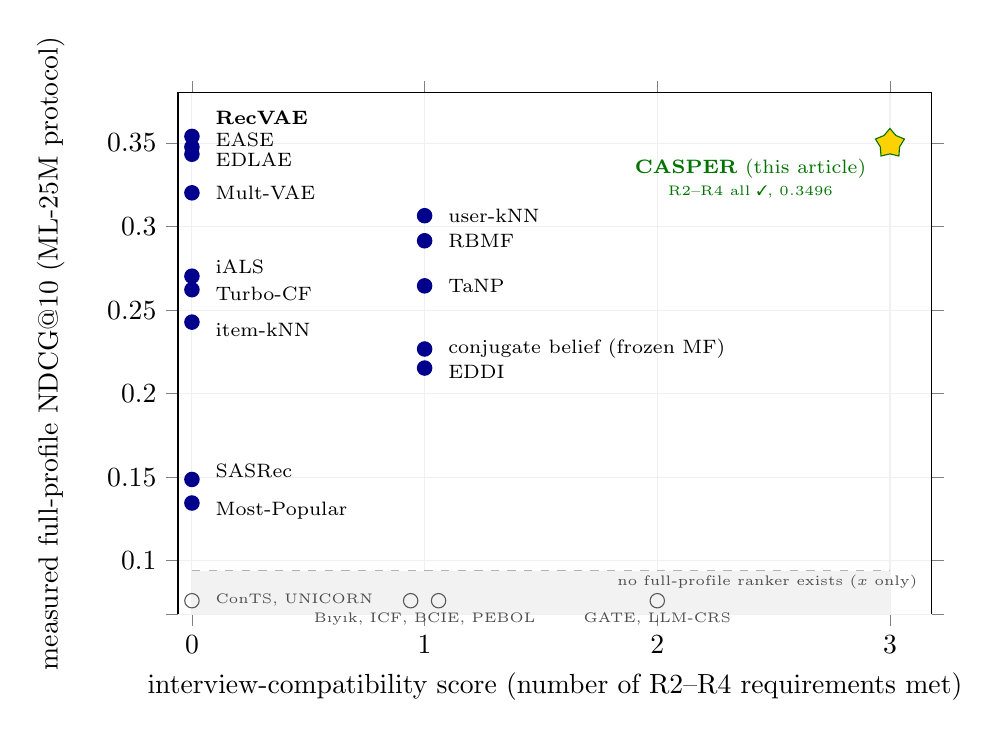
\begin{tikzpicture}
\begin{axis}[
    width=0.92\linewidth, height=8.2cm,
    xlabel={interview-compatibility score (number of R2--R4 requirements met)},
    ylabel={measured full-profile NDCG@10 (ML-25M protocol)},
    xmin=-0.06, xmax=3.18, ymin=0.068, ymax=0.38,
    xtick={0,1,2,3},
    ytick={0.10,0.15,0.20,0.25,0.30,0.35},
    ymajorgrids=true,
    extra y ticks={0.068}, extra y tick labels={},
    grid=both, grid style={gray!12},
    axis line style={-Latex},
    tick align=outside,
    clip=false,
]
  \node[star,star points=5,draw=green!45!black,fill=yellow!85!red,minimum size=11pt,inner sep=0pt]
        at (axis cs:3.0,0.3496) {};
  \node[green!45!black,font=\scriptsize,align=center,anchor=north east] at (axis cs:2.94,0.3466)
        {\textbf{CASPER} (this article)\\{\tiny R2--R4 all \cmark, $0.3496$}};
  \addplot[only marks,mark=*,mark size=2.6pt,color=blue!55!black] coordinates {
    (0.0,0.1345) (0.0,0.1486) (0.0,0.2428) (0.0,0.2622) (0.0,0.2703) (0.0,0.3202)
    (0.0,0.3433) (0.0,0.3476) (0.0,0.3540)
    (1.0,0.2153) (1.0,0.2267) (1.0,0.2645) (1.0,0.2915) (1.0,0.3065)
  };
  \node[font=\scriptsize,anchor=west] at (axis cs:0.06,0.1300) {Most-Popular};
  \node[font=\scriptsize,anchor=west] at (axis cs:0.06,0.1540) {SASRec};
  \node[font=\scriptsize,anchor=west] at (axis cs:0.06,0.2380) {item-kNN};
  \node[font=\scriptsize,anchor=west] at (axis cs:0.06,0.2600) {Turbo-CF};
  \node[font=\scriptsize,anchor=west] at (axis cs:0.06,0.2760) {iALS};
  \node[font=\scriptsize,anchor=west] at (axis cs:0.06,0.3202) {Mult-VAE};
  \node[font=\scriptsize,anchor=west] at (axis cs:0.06,0.3400) {EDLAE};
  \node[font=\scriptsize,anchor=west] at (axis cs:0.06,0.3520) {EASE};
  \node[font=\scriptsize,anchor=west] at (axis cs:0.06,0.3650) {\textbf{RecVAE}};
  \node[font=\scriptsize,anchor=west] at (axis cs:1.06,0.3065) {user-kNN};
  \node[font=\scriptsize,anchor=west] at (axis cs:1.06,0.2915) {RBMF};
  \node[font=\scriptsize,anchor=west] at (axis cs:1.06,0.2645) {TaNP};
  \node[font=\scriptsize,anchor=west] at (axis cs:1.06,0.2267) {conjugate belief (frozen MF)};
  \node[font=\scriptsize,anchor=west] at (axis cs:1.06,0.2130) {EDDI};
  \fill[gray!10] (axis cs:0,0.068) rectangle (axis cs:3,0.094);
  \draw[gray!60,dashed] (axis cs:0,0.094) -- (axis cs:3,0.094);
  \addplot[only marks,mark=o,mark size=2.6pt,color=gray!70!black] coordinates {
    (0.0,0.076) (0.94,0.076) (1.06,0.076) (2.0,0.076)
  };
  \node[gray!60!black,font=\tiny,anchor=west] at (axis cs:0.06,0.0765) {ConTS, UNICORN};
  \node[gray!60!black,font=\tiny,anchor=north] at (axis cs:1.0,0.0745) {B\i y\i k, ICF, BCIE, PEBOL};
  \node[gray!60!black,font=\tiny,anchor=north] at (axis cs:2.0,0.0745) {GATE, LLM-CRS};
  \node[gray!60!black,font=\tiny,anchor=east] at (axis cs:3.16,0.0870)
        {no full-profile ranker exists ($x$ only)};
\end{axis}
\end{tikzpicture}
\Description{Scatter plot of measured full-profile NDCG@10 against the number of interview requirements each system meets; the accuracy corner sits at zero requirements, the elicitation corner at one or two with no accuracy number, and the instrument alone at three requirements and frontier accuracy.}
\caption{The gap map. $y$: measured full-profile NDCG@10 under the ML-25M protocol (\textsc{liang}). $x$: the number of R2--R4 marks a system carries in Table~\ref{tab:master}, a coarse ordinal capability count; R1 is excluded because accuracy is the $y$-axis. Filled markers are every system with a measured full-profile number under this protocol (Table~\ref{tab:master}); hollow markers in the grey strip cannot produce one by construction, so only their $x$ position is meaningful. Runnable-but-unmeasured systems are absent. The accuracy corner sits at $x{=}0$, every system with interview machinery sits at $x\ge1$ and reports no full-catalogue accuracy, and no published system exceeds $x{=}2$. The star is the instrument, the only measured point at both the frontier bar and full interview compatibility.}
\label{fig:gapmap}
\end{figure}

% =====================================================================
\subsection{What each near-miss fails}\label{sec:gap}
% =====================================================================

No single published system satisfies all of $\{$R1 $\wedge$ R2 $\wedge$ R3 $\wedge$ R4$\}$. The closest near-miss is \citet{biyik2023soft}, which fails R1 (a $d{=}50$ ALS two-tower rather than a certified RecVAE-class recommender, with no full-catalogue accuracy reported) and gives only an approximate, ``generally not Gaussian'' posterior; it fails R2 in the sense that decides it, a per-concept supervised probe over a closed tag list rather than an open vocabulary. Every other candidate fails R3 or R4.

\paragraph{Where each near-miss falls short.}
\begin{itemize}[leftmargin=1.4em,itemsep=2pt]
  \item \textbf{\citet{biyik2023soft}} hold part of R2 (items and soft attributes both enter as directions) over a \emph{frozen} item tower; they train the CF model and the attribute directions separately, as we do. \emph{Fails R1}: a $d{=}50$ ALS two-tower, with accuracy reported on their own elicitation task (in-simulator top-$|S|$ agreement over 16 users, slates of 5), not the EASE/RecVAE bar. \emph{Fails R2} in the sense that decides it: the directions are per-attribute supervised probes over an enumerated tag list, each a logistic regressor fitted from labelled positive and negative items and trained for the 164 most frequent tags, so the vocabulary is fixed before the user arrives. R4 is approximate (sampled EVOI over a non-Gaussian posterior). This is the closest prior system, and the separation is (a) an open vocabulary through one global adapter with no per-concept supervision, (b) the R1 accuracy bar on a shared full-catalogue protocol, (c) exact rather than approximate conjugacy where a belief is maintained.
  \item \textbf{ConTS}~\citep{li2021seamlessly} holds R3 and a unified item/attribute action space. It fails R2, its attribute schema being a fixed categorical, and R1, being a bandit over arms rather than a full-profile encoder.
  \item \textbf{EDDI / Partial-VAE}~\citep{ma2019eddi} holds R3 and set input. It fails R1, having no full-catalogue ranking, and R2, its feature set being fixed.
  \item \textbf{RecVAE / EASE}~\citep{ren2020recvae,steck2019ease} hold R1. They fail R2 and R4, an item-only indicator basis admitting neither a concept nor a signed value, and R3, being point estimates.
  \item \textbf{PEBOL}~\citep{austin2024bayesian} holds R3 and R2, its LLM-extracted aspects being an open vocabulary. It fails R1, having no full-profile ranking, and R4, a yes/no answer carrying no intensity. Its belief is per item rather than a shared user covariance.
  \item \textbf{SASRec / BERT4Rec}~\citep{kang2018sasrec,sun2019bert4rec} re-encode the sequence at inference. They fail R2, R3 and R4: item-only, order-sensitive, point estimates, and non-monotone, since a later token can reorder everything. BERT4Rec's fold-in advantage also carries a replicability caveat~\citep{petrov2022replicability}.
\end{itemize}

\paragraph{The three legs an item-indicator basis cannot carry.}
Three input channels have no faithful encoding in the item-indicator basis of every R1-bar model. (i) Graded and signed per-entity values: the basis has no sign and no magnitude, and a dislike is not representable as a negative one-hot without changing the likelihood. (ii) Concepts whose vocabulary is not fixed when the model is fitted: a column exists only for an entity present at fit time. (iii) Arbitrary continuous direction tokens. Folding these as linear observations in a frozen latent is the one leg of the conjunction we find nowhere in the literature.

One obvious reduction exists, and its limits decide which of these channels is impossible and which is merely lossy. A concept whose members are all in the catalogue can be approximated by a weighted indicator over those members, and that vector feeds EASE or RecVAE without adding a column. Two bounds apply. The first applies to every concept: a nonnegative indicator has no encoding for a negative answer, since ``I dislike westerns'' is not expressible as a weighted bag of westerns, whatever the weights, because the basis carries no sign. The same limit is what the critiquing literature runs into (Section~\ref{sec:concept:lineage}), and it is what our own sign contrast measures directly ($+0.2096$, CI $[+0.1986,+0.2208]$). The second bound is absolute and applies to a narrower set: for a concept coined after the model was fitted, for a phrase with no curated counterpart, or for a direction a policy emits, there are no member columns to weight, so no reduction exists at any fidelity. An item-indicator model can be extended with a concept, as a pseudo-item column or an extra input unit, but only by adding a column, and a column is fixed when the model is fitted (Section~\ref{sec:setup:columns}). Our interface takes a direction $\bphi\in\R^{d}$ and a value, so any entity with an embedding is a legal observation at inference: a paraphrase, a concept coined after deployment, or a continuous direction emitted by a policy. This is what we mean by channel-agnostic, and it is a property of the interface.

\subsection{Feasibility and necessity of the conjunction}\label{sec:gap:why}

One objection to the analysis above is that the conjunction is inexpensive to satisfy: take a frontier recommender, carry a conjugate belief beside it, and the grid is complete. Three considerations tell against this.

\emph{Most of the frontier has nothing to carry a belief over.} A belief over a user latent needs a user vector in a dense latent and a direction in that latent to serve as a meaningful query. EASE has neither: its parameters are an item--item weight matrix and its ``user'' is the raw interaction row, one coordinate per catalogue item. There is no low-dimensional taste vector to be uncertain about and no direction to read $w^\top\bSigma w$ along. The same holds for EDLAE and for the training-free graph filters. For the closed-form models, which make up most of the accuracy corner, the construction is undefined. It is available to the amortised-encoder family, and that is where we build it.

\emph{Where it is available, it carries a cost.} Such a layer has to leave full-profile accuracy exactly intact, which is a property to be measured: our empty interview reproduces the frozen decoder's ranking identically (Spearman $1.0000$, $|\bmu_0|=0$), and the obvious alternative, ranking on a conjugate accumulator's mean, forfeits roughly $0.12$ full NDCG (Section~\ref{sec:method}). Nor does a dense latent accept concepts merely because it is dense: a raw concept centroid ranks its own member items at AUC $0.44$, below chance, and only whitening makes it a direction ($0.94$). 

\emph{And the reason to pay is that policy conclusions are not portable across recommenders.} This is the argument for an instrument, and it is empirical. On a strong ingestion model, differences between question-selection strategies compress: a random question from an answerable bank matches popularity-ranked items at $q{=}1,2,4,8$ and loses only at $q{=}16$; a one-level adaptive probe pays $+0.0015$ full (CI $[+0.0007,+0.0024]$); and an uncertainty-guided selector beats random by $+0.0036$ at the largest budget alone. A weaker recommender leaves more of the work to the question, so the same strategy gap measured there is larger and, if strategies are affected unequally, need not preserve the ordering. A policy result obtained on a weak recommender therefore carries an unknown amount of the recommender's own behaviour, which is the confound an instrument exists to remove, and Section~\ref{sec:res:inversion} shows it doing so.

\paragraph{On what the elicitation literature reports.} Cold-start MRR over a hundred-item shortlist, top-$|S|$ agreement with a posterior, and turn counts to a success state all measure a system on a task it would not perform in service. Full-catalogue NDCG is the only number in which an elicitation gain and a recommender weakness are on the same scale, and a policy improvement measured on a shortlist may not hold over $18{,}359$ candidates. We therefore treat a blank accuracy column as missing evidence rather than as a difference of emphasis.

% =====================================================================
\section{The Instrument}\label{sec:method}
% =====================================================================

The design follows from the gap analysis: use the shallow frozen recommender that already holds the accuracy corner (R1; the frontier has been flat since 2019, so a deeper model is not warranted), and add over its frozen latent a permutation-invariant set encoder that folds an evidence set of any length to a point (R2, R3), with every channel entering as a direction paired with a value (R4). Two trained components consume those pairs: the set encoder itself, which takes item evidence, and a gated operator, which takes concept evidence (Section~\ref{sec:concept:fold}). They are separate operators, and what is shared is the representation, not the code path: any entity with an embedding in the frozen latent can be written as one observation, so a single evidence set may mix channels. Figure~\ref{fig:architecture} summarises the interface.

\subsection{The frozen base recommender}
The base model is a certified shallow recommender, our RecVAE realisation~\citep{ren2020recvae}, trained once on the full catalogue and then frozen. It exposes (a) item factor rows $\Q_i\in\R^{d}$, (b) a decoder read-out $s_i(\uu)=\Q_i^\top\uu + \beta_i$ with a learned bias $\beta_i$, and (c) the encoder that maps a full interaction set to a latent. The decoder, its item factors and its bias are never updated; what is trained over them is the set encoder described below, and the whole model is frozen once that training is complete. Freezing is the guarantee that R1 is a property of the base model, not of the fold placed over it. It is a design choice we share with the soft-attribute line: \citet{gopfert2024cav} are explicit that ``we do not use the tag data when training the collaborative filtering model'', and \citet{biyik2023soft} train the CF model and the attribute directions separately. We do not extend the linear basis with concept columns (that stays in the item-indicator world and fails R2, because the vocabulary would again be fixed when the model is fitted), nor retrain the recommender to accommodate a channel, which would put R1 back at risk for no stated gain. \paragraph{Architecture and training of the set encoder.} The set encoder is a permutation-invariant network of the deep-sets form over the frozen $d{=}200$ latent. Each item observation enters as the item's own embedding, modulated by a learned scale and shift indexed by its half-star level (ten levels, $0.5$ to $5.0$ stars). The modulated embeddings pass through a token network of width $512$ and are sum-pooled. A residual network of the same width then maps three inputs to a shift of the latent: the pooled sum, the frozen RecVAE encoder's mean on the liked tokens, and the answered count. The weight on that anchor is gated by the number of answered items. A separate branch of the same form reads items that were asked about but not rated, so that exposure is not encoded as a weak dislike, and a learned prior latent supplies the belief with no evidence. The residual network's last layer, the exposure branch's last layer and the prior are zero-initialised, so at initialisation the encoder is the frozen base model exactly and every departure from it is driven by the loss. The trainable parameters number $1.07$ million against the frozen decoder. Training draws evidence sets from the training users' fold-in histories under a curriculum. The curriculum mixes full profiles, dropout-thinned profiles, short interviews of at most eight answered items in which unanswerable questions arrive as refusal tokens, and empty or single-answer sets. The objective is the multinomial negative log-likelihood of each user's held-out target items under the frozen decoder, with a smaller learning rate on the warm-started parameters than on the new branches. One run was trained; the checkpoint was selected on the validation users by full NDCG@10 and scored once on the test users. The selected model scores $0.3496/0.2491$ full/tail on the held-out test cohort and reproduces the frozen decoder exactly at the empty interview (Section~\ref{sec:res:battery}). It is this checkpoint that every channel below is folded into, and it is frozen for everything that follows.

\subsection{Channel-agnostic observations: one representation, one form of observation}
Every channel supplies the same kind of thing. An observation is a pair
\begin{equation}\label{eq:obs}
  (\bphi_j,\,y_j)\ \in\ \R^{d}\times\R,
\end{equation}
a direction $\bphi_j$ in the frozen latent and a value $y_j$, and it is this that makes the channel set open (R2). Any entity with an embedding is expressible as an observation, which is what no item-indicator model can say.

\begin{figure}[t]
\centering
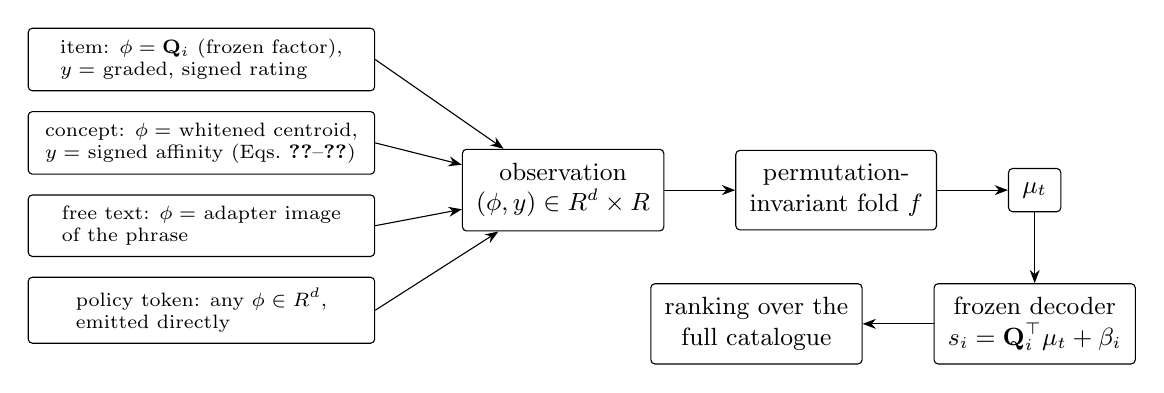
\begin{tikzpicture}[
  chan/.style={draw, rounded corners=1.5pt, align=left, font=\scriptsize, inner sep=4pt, minimum width=44mm},
  box/.style={draw, rounded corners=1.5pt, align=center, font=\small, inner sep=5pt},
  >=Stealth]
  \node[chan] (it) {item: $\bphi=\Q_i$ (frozen factor),\\ $y=$ graded, signed rating};
  \node[chan, below=2.5mm of it] (co) {concept: $\bphi=$ whitened centroid,\\ $y=$ signed affinity (Eqs.~\ref{eq:sel}--\ref{eq:val})};
  \node[chan, below=2.5mm of co] (tx) {free text: $\bphi=$ adapter image\\ of the phrase};
  \node[chan, below=2.5mm of tx] (po) {policy token: any $\bphi\in\R^{d}$,\\ emitted directly};
  \node[box, right=11mm of co.east, yshift=-6mm] (obs) {observation\\ $(\bphi,y)\in\R^{d}\times\R$};
  \draw[->] (it.east) -- (obs);
  \draw[->] (co.east) -- (obs);
  \draw[->] (tx.east) -- (obs);
  \draw[->] (po.east) -- (obs);
  \node[box, right=9mm of obs] (fold) {permutation-\\invariant fold $f$};
  \draw[->] (obs) -- (fold);
  \node[box, right=9mm of fold] (mu) {$\bmu_t$};
  \draw[->] (fold) -- (mu);
  \node[box, below=9mm of mu] (dec) {frozen decoder\\ $s_i=\Q_i^{\top}\bmu_t+\beta_i$};
  \draw[->] (mu) -- (dec);
  \node[box, left=9mm of dec] (rank) {ranking over the\\ full catalogue};
  \draw[->] (dec) -- (rank);
\end{tikzpicture}
\Description{Block diagram: four channels (item, concept, free text, policy token) each produce an observation pair of a direction and a value; a permutation-invariant fold maps the set of observations to a latent point; the frozen decoder ranks the full catalogue from that point.}
\caption{The channel-agnostic interface. Every channel reduces to the same form of observation, a direction in the frozen latent paired with a value; the permutation-invariant fold maps the evidence set to a point $\bmu_t$, and the frozen decoder ranks the catalogue. The item factors and the decoder belong to the certified recommender and are never updated, which is what makes R1 a property of the base model; the three lower channels are the legs an item-indicator basis cannot carry (Section~\ref{sec:gap}).}
\label{fig:architecture}
\end{figure}

\paragraph{Why a learned fold rather than a closed-form one.} A closed-form conjugate accumulator over the frozen factorisation is itself a legal ranker (score item $i$ by $\Q_i^\top\bmu_t+\beta_i$), and it would make one uniform fold serve every channel. We measured that option: ranked by its accumulated mean it reaches full/tail NDCG@10 $0.2267/0.1300$ under our protocol, against $0.3496/0.2491$ for the learned fold (Table~\ref{tab:master}). Uniformity therefore costs roughly $0.12$ full NDCG ($0.3496-0.2267$), forfeiting R1, which is why the instrument folds with a learned set encoder and pays for the extra operator.

The channels are:
\begin{itemize}[leftmargin=1.4em,itemsep=1.5pt]
  \item \textbf{Items.} $\bphi_j=\Q_i$, the frozen item factor. A graded or signed answer sets $y_j$; a dislike is a negative $y_j$ along the same direction, representable because the observation model \eqref{eq:obs} has a sign and a magnitude.
  \item \textbf{Out-of-catalogue concepts.} $\bphi_j$ is a concept direction in the latent (a whitened centroid of member factors, or a text-adapter image of the concept), folded like an item; no catalogue column is required.
  \item \textbf{Entities and free text.} An embedding is projected into the latent by a fixed adapter and folded identically.
  \item \textbf{Continuous direction tokens.} A policy may emit any $\bphi_j\in\R^{d}$ directly; the fold does not distinguish it from a catalogue entity.
\end{itemize}

\paragraph{Any direction is a legal observation.} The signed/graded leg is delivered and measured (R4, Figure~\ref{fig:gradedcurve}). The concept leg is delivered over the genome vocabulary (Section~\ref{sec:concept}). The third leg, an arbitrary direction including one for an entity that has no catalogue column and was never seen in training, is a property of the interface: everything downstream of Eq.~\eqref{eq:obs} consumes a pair $(\bphi,y)$, so any entity with an embedding is admissible. We illustrate that concretely. Each of the $1{,}031$ genome concepts has a direction in the latent and a name in English, so those pairs determine a single global linear map from a frozen general-purpose sentence encoder into the frozen latent, in closed form. We fit it on a random $80\%$ of the concepts and ask what happens to the $20\%$ it never saw: for a held-out concept, the direction predicted from its name alone recovers the top of that concept's own item ranking more than $300\times$ more often than chance ($0.167$ top-10 overlap against a $0.0005$ random baseline; cosine $0.638$ to the true direction). No per-concept probe is fitted, no inventory is consulted, and nothing is retrained: a phrase becomes a direction by one matrix multiplication.

Because the map is defined on any string, it also accepts phrases that are not in the concept vocabulary. To make that meaningful, each phrase in Table~\ref{tab:freetext} is screened against the vocabulary two ways (no genome tag occurs as a whole-word substring of it, and no concept sits within cosine $0.6$ of it), and we print the closest concept we hold, so the reader can see how far the phrase sits from anything curated. The screen rejects ``revenge served slowly'', ``loneliness in a big city'' and ``a detective who drinks too much'', because \emph{revenge}, \emph{loneliness} and \emph{detective} are themselves genome tags. The last row is the clearest case: the nearest concept in the entire vocabulary to ``movies about grief'' is \emph{feel good movie}, tonally its opposite, and the phrase's direction shares none of its top ten items with that concept's curated direction; the phrase is placed by its own meaning, not snapped to the closest thing on a list. Phrases whose meaning the genome vocabulary does not carry at all (``set entirely inside one room'') return lists we would not defend. We present this as an illustration of what the interface permits, not as a contribution to mapping language into collaborative latents, a question with an established literature in which attribute directions are obtained either by per-concept supervised probes~\citep{gopfert2024cav,biyik2023soft} or by per-attribute corpus retrieval~\citep{balog2021softattr}. Fitting such a map well is a research direction this architecture opens.

\begin{table}[t]\centering\small
\setlength{\tabcolsep}{5pt}
\begin{tabular}{p{4.2cm}p{2.0cm}c p{5.4cm}}
\toprule
free-text phrase & nearest concept & cos & top of the returned ranking \\
\midrule
``the quiet dignity of losing'' & \emph{redemption} & $0.47$ & Umberto D.; Tyson; Red Army; Days of Glory \\
``people trapped by a decision they made years ago'' & \emph{history} & $0.39$ & Music Box; Judgment at Nuremberg; Missing \\
``two people talking for the whole film'' & \emph{dialogue} & $0.54$ & Sweet Smell of Success; Trouble in Paradise \\
``movies about grief'' & \emph{feel good movie} & $0.54$ & Rachel, Rachel; Mean Creek; The Woodsman \\
\bottomrule
\end{tabular}
\caption{Free-text phrases with no curated counterpart. Four free-text phrases, each screened against the $1{,}031$-concept vocabulary two ways (no genome tag occurs as a whole-word substring, and no concept sits within cosine $0.6$), with the nearest concept we hold printed so the distance from anything curated is visible. Directions come from the single global map fitted on $80\%$ of the concepts; nothing is retrained or looked up.}
\label{tab:freetext}
\end{table}

\paragraph{The observation is independent of its provenance.} Eq.~\eqref{eq:obs} reads a pair $(\bphi,y)$ and is indifferent to where it came from: a user who volunteers ``I'm in the mood for something about grief'' has supplied a direction and a positive value, which folds exactly as an answer to a question we posed would. The same holds for a critique after a recommendation (``less bleak than that'') and for a direction a continuous policy emits and never renders as language. An item-indicator model cannot accept any of these, because none has a column; a model with a curated attribute list can accept only those a curator anticipated. A user-initiated request folds the same way, and is available because of R2. We have not evaluated proactive requests here, and the quality of any such interaction would rest on the text adapter whose limits are set out above.

\begin{figure}[t]
  \centering
  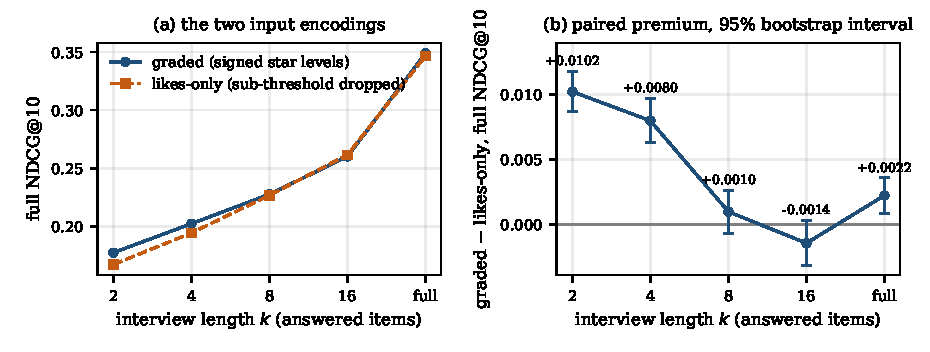
\includegraphics[width=0.98\linewidth]{fig_graded_curve_tors.pdf}
  \Description{Two panels. Left: full NDCG@10 against interview length for graded and likes-only input; the graded curve is above the likes-only curve at two and four questions and the two coincide from eight questions onward. Right: the paired premium of graded over likes-only with its bootstrap interval, positive at two and four questions, indistinguishable from zero at eight and sixteen, and small but positive at the full profile.}
  \caption{Graded input helps over binarised input, most on the short interview. ML-25M interview harness, full NDCG@10 against interview length $k$. The same revealed set is fed two ways: \emph{graded} (real signed star levels) and \emph{likes-only} (sub-threshold answers dropped, what a positive-only model such as RecVAE does at $r{>}3.5$). Panel (b) plots the paired premium with its $95\%$ bootstrap interval over the $10{,}000$ users: positive with an interval excluding zero only while evidence is scarce, $+0.0102$ at $k{=}2$ (CI $[+0.0087,+0.0118]$) and $+0.0080$ at $k{=}4$ (CI $[+0.0063,+0.0097]$), indistinguishable from zero at $k{=}8$ and $k{=}16$, and $+0.0022$ (CI $[+0.0008,+0.0036]$) at the full profile, where the graded history is folded against the likes-only history. The extra bits a star carries matter most when few items are known. The separate full-profile comparison on identical support ($+0.0039$) is in Section~\ref{sec:res:battery}.}
  \label{fig:gradedcurve}
\end{figure}

% =====================================================================
\section{The Concept Channel}\label{sec:concept}
% =====================================================================

The out-of-catalogue concept leg is the most demanding of the three. It has no catalogue column, no interaction count and no sign in the item-indicator basis, so we set it out in full: how a concept answer becomes an observation pair $(\bphi_c, y_c)$ for the fold of Eq.~\eqref{eq:obs}; where each piece sits in the published record, so that we claim only the conjunction; and why this channel forces the battery to gate what a deployed interview elicits, not only what the operator can express.

\subsection{A signed, exposure-corrected affinity estimator}\label{sec:concept:est}

A concept answer must supply the value $y_c$ that Eq.~\eqref{eq:obs} reads along the concept direction. We want that value to be \emph{signed} (a user can dislike ``horror'', not merely fail to like it), \emph{popularity-corrected} (a concept made of blockbusters must not read as universal affinity), \emph{volume-corrected} (a heavy watcher must not read as liking everything) and \emph{confidence-bearing} (a concept the user has plausibly never been exposed to is a refusal, not a dislike). Two estimators, an implicit and an explicit one, combine to meet this.

Let $\mathcal I_u$ be the user's watched set, $p_i$ the catalogue marginal of item $i$, and let concept $c$ have member set $M_c$. Write $n_c=|\mathcal I_u\cap M_c|$ for the user's watched members and $e_c=|\mathcal I_u|\cdot\pi_c$ for the number expected under the user's volume times the concept's popularity $\pi_c=\sum_{i\in M_c}p_i$. The implicit \emph{selection} estimator is the add-$\tfrac12$ log watch-lift
\begin{equation}\label{eq:sel}
  \mathrm{SEL}(u,c) \;=\; \log_2\frac{n_c+0.5}{e_c+0.5}
  \;\;\approx\;\; \mathrm{PMI}(u,c),
\end{equation}
which is the pointwise mutual information between the user and the concept: the denominator's $\pi_c$ divides out concept popularity, and forming $e_c$ from the user's own volume divides out user activity, so SEL is positive for genuine affinity, near zero for popularity-explained co-occurrence, and negative for avoidance. Its normalised form, $\mathrm{NPMI}=\mathrm{PMI}/(-\log_2 \hat p_{uc})\in[-1,1]$, corrects PMI's small-count inflation and yields a bounded, comparable score. The explicit \emph{value} estimator is a support-shrunk signed rating residual,
\begin{equation}\label{eq:val}
  \mathrm{VAL}(u,c) \;=\; \frac{n_c}{n_c+\lambda}\;\bar r^{\,\mathrm{res}}_{uc},
  \qquad \lambda=3,\qquad
  \bar r^{\,\mathrm{res}}_{uc}=\frac{1}{n_c}\!\!\sum_{i\in\mathcal I_u\cap M_c}\!\!\bigl(r_{ui}-\bar r_i\bigr),
\end{equation}
the mean rating the user gives the concept's members above each item's own mean, shrunk toward zero by the factor $n_c/(n_c+\lambda)$ so that a one-film opinion counts for little. Both estimators are signed and combine into a four-band answer: a \emph{graded like} (SEL/VAL band above the neutral zone), a \emph{neutral} (indistinguishable from exposure), a \emph{graded dislike} (band below), and a \emph{refusal} issued exactly when the expected support falls below a threshold, $e_c<\tau$, when the user has plausibly never been exposed to the concept and no answer should be forced.

\paragraph{Lineage.} Every piece is established prior art. The log-lift \eqref{eq:sel} is PMI/NPMI, the standard popularity-corrected association score. Reading a magnitude of implicit consumption as evidence is the implicit-confidence template of \citet{hu2008collaborative}, except that there the count re-enters only as a loss confidence weight, never as a sign, which is the assumption our signed estimator breaks. The principled account of why a non-watch is not a dislike is ExpoMF~\citep{liang2016expomf}: it separates a latent exposure variable from preference, so that non-consumption is modelled as ``not exposed'' or ``exposed and disliked'', the account our refusal band ($e_c<\tau$) and popularity-corrected $e_c$ approximate cheaply and in closed form. The unbiased-learning route to the same correction is attribute-level exposure propensity~\citep{qin2020attributepropensity}, the heavier, variance-prone alternative to our moment estimator. Calibrated recommendation~\citep{steck2018calibrated} builds a user's normalised genre distribution $p(g\mid u)$, the closest widely used ``concept profile'', but a distribution that sums to one encodes relative emphasis only and cannot express dislike, which is the expressive gap $\mathrm{SEL}<0$ fills.

\paragraph{Why the implicit channel, quantified.} We decompose informativeness by a per-concept linear fit of the oracle concept affinity onto each candidate answer ($R^2$). The implicit watch-lift dominates: SEL explains $0.376$ of the affinity variance, and the explicit rating residual VAL a further $+0.042$ (SEL$+$VAL $0.398$). An LLM-elicited ordinal answer explains only $0.017$, so the implicit channel outperforms the explicit LLM answer by roughly $22\times$. Because SEL is built from raw watch counts and item marginals, it uses no recommender geometry, so this signal is non-circular by construction. This is the evidence that the concept channel's value is worth carrying signed rather than as a membership indicator; the decomposition is an informativeness measurement, not an interview curve.

\subsection{The fold operator: whitened directions and a gated fold-to-point}\label{sec:concept:fold}

The direction $\bphi_c$ must separate the concept's members from non-members. A raw member centroid fails this: a shared popularity component (random concept pairs have cosine $\approx 0.5$) masks the genre geometry. Removing it, by centring the member factors and stripping the top principal component, the all-but-the-top whitening of \citet{mu2018allbutthetop}, turns the centroid into a usable direction: concept-membership discrimination through the frozen decoder rises from AUC $0.44$ (raw, below chance) to $0.94$ (whitened). We therefore take $\bphi_c$ to be the whitened member centroid, IDF-weighted by $1/\log(1+|M_c|)$ so broad genres do not dominate.

The operator that consumes $(\bphi_c,y_c)$ is the design decision, and the two candidate families separate under ablation. An \emph{additive-union} operator scores each item by summing concept contributions on a popularity floor, $s_i=\beta_i+\sum_c w_c\,\langle \W_d\Q_i,\bphi_c\rangle$. It has the right monotonicity floor (an empty interview scores exactly $\beta_i$) but the wrong composition: it scores the union of directions, so correlated sibling concepts (``dark'', ``gritty'', ``noir'') re-add the same acclaim axis and over-count. Measured against a no-answer intercept of $0.1279$ full NDCG@10, the additive channel peaks early (about $+0.011$ at two answers) and then declines as answers accumulate, reaching $0.0991$ at eight answers, below the intercept. A \emph{trained gated fold-to-point} operator fixes this by folding the answers into the latent itself and letting the frozen decoder apply the full collaborative (intersection) structure:
\begin{equation}\label{eq:cfold}
  \uu \;\leftarrow\; \uu + \sigma\!\bigl(g([\uu;\bphi_c;y_c])\bigr)\;\odot\;h([\uu;\bphi_c;y_c]),
\end{equation}
with the gate $g$ and the delta MLP $h$ zero-initialised, so that at initialisation $\uu$ is unchanged and R1 survives, and the accumulated shift norm-capped per user. In the operator ablation it is monotone in the number of answers to eight ($0.1759/0.0841$ full/tail at eight answers, up from $0.1322/0.0503$ at one) and redundancy-robust: feeding it eight \emph{correlated} top-SEL concepts still reaches $0.1685/0.0906$, above its four-answer level ($0.1572/0.0777$), exactly where the additive-union operator degraded. The ablation also settles the member-lift tension of Section~\ref{sec:reqs}: the additive-union operator reaches member AUC $0.820$ but falls below the intercept, while the gated fold sits at $0.626$ and reaches $0.1759$. The gated fold is the concept operator we adopt; Eq.~\eqref{eq:cfold} is the concept-channel instantiation of the channel-agnostic fold of Section~\ref{sec:method}.\footnote{The operator ablation was run on an earlier checkpoint, so the numbers in this paragraph are that checkpoint's. It settles the operator choice rather than the absolute level: additive-union declines where the gated fold stays monotone and redundancy-robust. The deployed numbers are in Section~\ref{sec:res:concept}.}

\subsection{Lineage, and why critiquing is not channel-open}\label{sec:concept:lineage}

The skeleton, an attribute as a latent direction folded by a belief update over a frozen factor space, is established, and we claim none of it in isolation. \citet{biyik2023soft} treat a soft attribute as a concept-activation-vector direction and fold signed answers into a Gaussian belief; M\&Ms-VAE folds a rating posterior and an attribute posterior over one latent by a product-of-experts merge~\citep{antognini2021mmvae}; its successor adds an independent signed critique axis through learned positive/negative conditioning tokens, and reports that negative critiquing saturates after about five turns~\citep{antognini2022posneg}, a concrete ceiling for any signed-attribute channel, consistent with our own concept curves. BK-VAE folds keyphrase-activation-vector directions by a Bayesian critiquing step~\citep{yang2021bkvae}; the gate and MLP of Eq.~\eqref{eq:cfold} are a per-token generalisation of FiLM conditioning~\citep{perez2018film}, which a single global affine cannot do because it would apply the same modulation to item and concept tokens alike. The decision to freeze the recommender rather than co-train a concept head is a direct reading of the result that a separately trained critique head costs recommendation accuracy~\citep{wu2019dlc,luo2020cevae}.

Critiquing is the one line that appears to accept free-form input and therefore appears to satisfy R2. It does not: across the family the critique is defined as a one-hot indicator over a closed set. DLC embeds a one-hot keyphrase~\citep{wu2019dlc}; LLC states that critiques ``are encoded as one-hot keyphrase indicators''~\citep{luo2020llc}; CE-VAE defines ``a one-hot vector with keyphrase length $s$''~\citep{luo2020cevae}; M\&Ms-VAE uses ``a one-hot vector of length $|K|$''~\citep{antognini2021mmvae}; Bot Play accumulates over a fixed aspect set~\citep{li2021botplay}. The vocabularies are small, $40$ or $75$ keyphrases for catalogues of thousands of items, and where the representation is continuous, the continuity is downstream of an argmax. The lineage is older than the neural work and has the same shape: FindMe's tweaks are fixed operations on a slot-value schema~\citep{burke1996findme}, and Chen and Pu's survey defines a unit critique as one that ``can only constrain over a single feature at a time''~\citep{chenpu2012critiquing}. The nearest counterexample is BCIE, whose critique is a knowledge-graph fact drawn from about $57$k entities and $46$ relations~\citep{toroghi2023bcie}, three orders of magnitude larger and the case that most qualifies our claim on R2, but the fact must still be one the system surfaced. What none of these holds jointly is the conjunction this channel occupies: continuous, out-of-catalogue concept directions (a whitened centroid or a text-adapter image, with no per-attribute probe to train), driven by a signed, exposure-corrected implicit affinity (Eqs.~\eqref{eq:sel}--\eqref{eq:val}), folded over a frozen, certified, frontier-accuracy recommender.

\subsection{Why testing the operator is not enough}\label{sec:concept:deploy}

A gate on what an operator \emph{can} express must be paired with a gate on what the deployed system \emph{does} express, and the concept channel is where the distinction matters. The fold of Eq.~\eqref{eq:cfold} is sign-capable: negating every concept answer of a user's full concept profile moves NDCG by $-0.2012$ with an interval excluding zero (the item-history counterpart in Table~\ref{tab:battery} is $-0.2953$), so the concept channel passes R4's sign-flip test on its own operator. But that certifies the operator, not the interview. Driven down a realistic, user-independent question bank, most concept answers are weak positives, and an answer model that never emits a negative can accumulate them until the ranking drifts below the no-answer intercept while every capability check still passes. We therefore evaluate the channel under a \emph{spend-on-ask budget}: a fixed, user-independent bank under a per-question budget where every question spends budget whether or not it is answered, scored at the endpoint against the intercept (R3's fixed-bank setting). The acceptance form of the concept channel is not ``can the operator express dislike'' but ``does the realisable interview stay above the no-answer intercept at budget''. This is the criterion the signed four-band estimator of Section~\ref{sec:concept:est} is built to satisfy, and it is checked by three pre-specified criteria: the signed answer must beat a positive-only clip of the same answer at budget; a popularity-only answer built from the user's volume and the concept's popularity must reproduce none of the gain; and permuting the answer values across concepts must collapse it. Section~\ref{sec:res:concept} reports all three. We therefore accept the concept channel on its endpoint under the spend-on-ask budget, not on what its operator can express.

The signed concept fold is a trained fold-to-point over the frozen certified recommender rather than a set of concept tokens trained into the recommender itself. That choice is what leaves R1 intact without re-establishing it: the fold's final layer is zero-initialised, so at an empty interview it is bit-identical to the recommender on the full profile, and no concept training can put the certified full-profile number at risk. It also keeps the channel replaceable: a better concept operator can be fitted and swapped without retraining or recertifying the recommender, which is what makes this an instrument.

% =====================================================================
\section{Experimental Setup}\label{sec:setup}
% =====================================================================

\subsection{Data and protocol}
All full-profile numbers are on MovieLens-25M under the strong-generalisation recipe of \citet{liang2018variational}, applied to the project catalogue. Items need at least 20 ratings, which gives a catalogue of $18{,}430$ films, of which $18{,}359$ occur in the training vocabulary. Ratings above $3.5$ count as likes, and users need at least five likes. The user-level split is $140{,}768$ training, $10{,}000$ validation and $10{,}000$ test users, with each held-out user's history divided $80/20$ into a fold-in and a target half (seed $98765$). The primary metric is NDCG@10 on the full catalogue and on the tail, the tail being the catalogue with the head items that carry the top third of training mass (190 items) masked out; tail NDCG is defined for the $9{,}281$ test users who hold at least one target outside the head, and every tail interval is over those users. NDCG@100 is secondary. Every model is scored with its own learned decoder bias rather than a popularity floor. All hyperparameters and checkpoints were selected on the validation users and scored once on the test users.

\paragraph{Statistics.} Every headline delta carries a paired per-user bootstrap confidence interval, $10{,}000$ resamples over the $10{,}000$ test users, on one shared harness; a difference is called separated when its interval excludes zero, and indistinguishable when it does not (Definition~\ref{def:tie}). Intervals are reported per cell without a family-wise correction. The claims that rest on a single interval are the R1 contrasts, whose tolerance was fixed in advance; every other claim in the article rests on directional consistency across budgets, metrics and controls rather than on one cell, and the controls of Table~\ref{tab:battery} are reported with the same intervals as the arms they qualify. Interview curves use the same test cohort: the fold-in half supplies the answers, the target half is scored, and the cold intercept of $0.1279/0.0192$ is the non-personalised read-out of the frozen decoder bias. ML-25M carries the Tag Genome, whose $1{,}031$ tags are the concept vocabulary.

\subsection{The certification bridge}\label{sec:bridge}
Our ML-25M protocol and the published bar are on different metrics and splits: our RecVAE realisation reaches full/tail NDCG@10 $0.3540/0.2497$ on ML-25M, whereas the published EASE and RecVAE numbers are NDCG@100 on the ML-20M strong-generalisation split. These are not comparable, and no R1 claim is made until the bridge is run. The bridge has two steps: (1) reproduce the published EASE and Mult-VAE/RecVAE numbers on the ML-20M split (NDCG@100, Recall@20/50) in our own code~\citep{steck2019ease,liang2018variational,ren2020recvae}; (2) port the certified recommender to the ML-25M harness and report full/tail NDCG@10 there. ML-20M stays in the loop because the 2018 split is a dependence on one protocol the whole full-profile literature reports on; ML-25M carries the genome tags the concept channel needs, so both are required, one for comparability and one for the channels.

On the ML-20M split our split statistics reproduce the published counts exactly ($9{,}990{,}682$ events, $116{,}677$ train users, $20{,}108$ items), and both anchor implementations reproduce their published values: EASE at NDCG@100 $0.4203$ against the reported $0.420$~\citep{steck2019ease}, and RecVAE at $0.4425$ against $0.442$, with Recall@20 ($0.4144$ against $0.414$) and Recall@50 ($0.5525$ against $0.553$) matching as well~\citep{ren2020recvae}. One closed-form and one neural reproduction to the third decimal certify that our split construction, metric implementation and both implementation families are faithful to the published protocol; every ML-25M baseline number therefore comes from certified code. Mult-VAE reaches $0.4223$ against the published $0.426$ ($-0.0037$; Recall@20 $0.3928$ against $0.395$, Recall@50 $0.5341$ against $0.537$), a near match, admitted as a bridged anchor and labelled as such. Mult-DAE fails, $0.3969$ against $0.419$, and rather than carry an uncertified implementation we drop it from the baseline bank. The same rule applied to ourselves costs something: our iALS lands at $0.358$ against the published WMF anchor of $0.386$, a larger miss than the one that disqualified Mult-DAE, so iALS is an uncertified floor rather than a bridged anchor. It keeps its measured row under the ML-25M protocol but is excluded from every claim that requires a certified comparator. Only EASE, RecVAE and, as a near match, Mult-VAE carry certified status, and the argument for the division stands on those.

\subsection{Baseline bank}
The bank has three tiers. \emph{Classic floors} that every curve must clear, which \citet{dacrema2019progress} demand: Most-Popular, Item-kNN as the strong simple baseline of \citet{cremonesi2010performance}, and PureSVD/iALS as cheap fold-in references. \emph{Full-profile frontier}, which decides R1: EASE and RecVAE as the bar, Mult-VAE as the canonical amortised anchor, EDLAE to confirm the frontier is flat, plus the graph-filter and sequence families (Turbo-CF, SASRec). \emph{Elicitation-compatible rivals}, which decide R3 and R4: EDDI for the set-encoder-plus-information-gain architecture, \citet{biyik2023soft} as the closest prior system, ConTS and BCIE for the conjugate-belief lineage, PEBOL as the principal preference-elicitation baseline, and Golbandi's node model, RBMF and TaNP as the interview consumers of Section~\ref{sec:res:inversion}. Per-row configuration, where a row required a choice: EDLAE at validation-selected $p{=}0.4$; Turbo-CF at validation-tuned $\alpha{=}0.5$, $s{=}1$, second order; EDDI early-stopped at epoch $46$ with epoch $31$ validation-selected; TaNP best-effort with its rating channel binarised; user-kNN, RBMF and the conjugate belief are best-effort cores of the elicitation-corner systems rather than their published systems. Our RecVAE follows the paper configuration. On this protocol RecVAE attains $0.3540/0.2497$, ahead of the closed-form leaders EASE ($0.3476/0.2441$) and EDLAE ($0.3433/0.2395$); the top of the table is a narrow band, RecVAE leading EASE by $+0.0064$ full. We therefore treat RecVAE as the bar, the strongest measured system and the conservative one to be held to. NDCG@100 orders the most accurate systems and the first six rows of the \textsc{liang} column identically, and reorders only the middle of the table, where RBMF, EDDI and the conjugate belief move. The values are RecVAE $0.4537$, ours $0.4492$, EASE $0.4375$, EDLAE $0.4330$, Mult-VAE $0.4303$, user-kNN $0.3958$, iALS $0.3700$, TaNP $0.3661$, Turbo-CF $0.3569$, RBMF $0.3533$, Item-kNN $0.3200$, EDDI $0.3110$, the conjugate belief $0.2883$, SASRec $0.2465$, Most-Popular $0.1975$.

\subsection{Answer provenance: what may not enter an answer}\label{sec:provenance}
An interview evaluation is only as trustworthy as the thing that answers it, and the failure mode is specific: if any quantity derived from the recommender reaches the answer, the interview curve measures the recommender recovering its own geometry rather than ingesting evidence. That inflates every downstream number without transferring to a real user, and it cannot be detected from the curve, because a circular answer model produces a curve of the shape a working one produces. We therefore treat the answer path as a protocol object, with a rule stated in advance and enforced in code.

\paragraph{The rule.} An answer may be computed only from the user's fold-in behaviour and from catalogue-level counts. An item answer is the user's own recorded rating; a concept answer is the signed log watch-lift of Eq.~\eqref{eq:sel}. Three things are excluded by construction, and each exclusion is asserted in code. \emph{No recommender-derived quantity}: no latent, factor, score, similarity or model-predicted rating enters an answer, and the answer path never reads the recommender. \emph{No target-half information}: answers are computed from the fold-in half only, so an answer cannot encode the held-out items it will be scored against. \emph{No oracle over unobserved preference}: where a user has no evidence about a concept, the estimator emits a refusal rather than an imputed preference.

Applied as a checklist, the rule sorts this literature into the simulators that satisfy it and those that do not. PEBOL's simulated user answers from the ground-truth item description~\citep{austin2024bayesian}, so the answer is a function of the target. Unified item-and-attribute conversational work assumes the user holds and reveals a clear preference over every attribute and item~\citep{deng2021unicorn}, which supplies an oracle exactly where a cold user has no evidence. Bandit-over-arms formulations draw answers from the same latent space the recommender ranks in~\citep{li2021seamlessly}, circularity. None of these is a careless choice; each is a reasonable simulator design. But each makes the resulting interview curve a statement about the simulator as much as about the method, and none would pass the rule above. We make no claim that our answers are what a person would say; the claim is narrower and checkable: whatever these answers are, they are computed independently of the model being evaluated.

\subsection{Why ``just add genre columns'' is not an alternative}\label{sec:setup:columns}
The obvious objection to the concept channel is that a concept could simply be appended to an item-only model as an extra column, a centroid-of-members pseudo-item in EASE or an extra input unit in RecVAE. The objection fails because of what the indicator basis can represent. EASE's item--item weight matrix is defined over a fixed column set and is obtained in closed form from the Gram matrix of exactly those columns; RecVAE's input layer has one weight vector per column. Adding a concept therefore means adding a column, and adding a column means refitting the model: the set of expressible concepts is frozen at training time. A paraphrase of an existing concept, a concept invented after deployment, a direction produced by snapping a continuous query to the nearest meaningful axis, none can be answered without retraining, because none has a column. No item-only baseline therefore appears in the mixed-channel comparison of Section~\ref{sec:res:concept}, because none can fold a concept at all, which is the architecture limit.

\subsection{Interview protocol}
Interview curves start every test user cold (no item history), pose questions from a bank, fold each graded answer through the instrument, and score the target half at each budget. Answers are read from the user's full graded fold-in history, sub-threshold ratings included, whereas the full-profile rows of Table~\ref{tab:master} read the \textsc{liang} likes; the two regimes are never compared with each other. Two intercepts appear in the results and are never compared across: the item-interview harness starts from $0.1279/0.0192$, the frozen decoder's non-personalised read-out, and the concept-channel protocol of Section~\ref{sec:res:concept}, which scores under its own pool, starts from $0.1277/0.0267$. ``No popularity floor'' means that a consumer that receives no answer ranks by its own empty-input output rather than backing off to a popularity ranking. The four bank rankings of Section~\ref{sec:res:concept} are \textsc{pop} (by the fraction of users who can answer), \textsc{entropy} (by the entropy of the four-way ask outcome: like, neutral, dislike, refusal), \textsc{polar} (by the entropy of the answer band among users who answer) and \textsc{expinfo} (\textsc{polar} weighted by the probability of an answer). Two bank regimes are used and named separately. The \emph{fixed bank} of R3 is a question set fixed in advance and filtered per user to answerable questions, isolating ingestion from availability. The \emph{spend-on-ask} regime of Sections~\ref{sec:res:inversion} and~\ref{sec:res:concept} uses a fixed, user-independent bank under a per-question budget in which an unanswered question still spends its turn; an item question is answerable when the user's fold-in half contains a rating for it, a concept question when the user's expected support clears the refusal threshold. Where the two channels are compared, the protocol is matched: the same cold users, the same held-out targets, the same budget, an unanswerable question spending the budget in either arm, and at zero questions the two arms bit-identical by construction. The instrument-dependence experiment of Section~\ref{sec:res:inversion} fixes the questions, users, answers, budget ($k{=}8$) and candidate pool (\textsc{native}) and varies only the consuming recommender.

\paragraph{Code and artefacts.} The split construction, every baseline and its tuning, the bridge, the certified checkpoint, the battery and the per-user score vectors behind every table are released at [repository URL to be added at submission], and will be archived on a permanent public store at acceptance.

% =====================================================================
\section{Results}\label{sec:results}
% =====================================================================

\subsection{RQ1: Strategy rankings invert with the recommender}\label{sec:res:inversion}

Everything above argues that a certified, interviewable recommender is buildable. This subsection shows it is necessary: without one, a comparison between elicitation strategies does not have a stable answer. \citet{rashid2008learning} report the order \textsc{helf} $>$ \textsc{entropy0} $>$ \textsc{popularity}. We ran all three under a fixed interview protocol (identical users, budget $k{=}8$, answer model, a question bank fixed in advance, no popularity floor) and varied only the recommender that consumes the answers. Table~\ref{tab:instrdep} reports six consumers: the instrument; the same RecVAE that sets the R1 bar, restricted to the likes among the asked items; and best-effort reconstructions of the node model at the core of Golbandi's tree, of RBMF, of a conjugate-Gaussian belief over a frozen factorisation, and of TaNP. Only the first two are run as designed, and every substitution in the other four is stated in Section~\ref{sec:related}.

\begin{table}[t]\centering\scriptsize
\setlength{\tabcolsep}{4pt}
\renewcommand{\arraystretch}{1.18}
\begin{tabular}{p{3.6cm}ccc l l}
\toprule
Recommender consuming the answers & \textsc{helf} & \textsc{ent0} & \textsc{pop} &
  Order & Ours $-$ row \\
\midrule
graded answers of 8 (all consumers) & $1.59$ & $3.10$ & $3.05$ & & \\
\midrule
\multicolumn{6}{l}{\emph{full NDCG@10}}\\
CASPER instrument (ours) & $.1892$ & $\mathbf{.2053}$ & $.1943$ & \textbf{E0 $>$ P $>$ H} & --- \\
RecVAE, likes-only~\citep{ren2020recvae}$^{\S}$ & $.1003$ & $.1718$ & $\mathbf{.1760}$ & \textbf{P $>$ E0 $>$ H} & $+.0293$ $[+.0267,+.0320]$ \\
Golbandi node model~\citep{golbandi2011adaptive}$^{\ddagger}$ & $\mathbf{.1948}$ & $.1686$ & $.1716$ & \textbf{H $>$ P $>$ E0} & $+.0105$ $[+.0072,+.0137]$ \\
RBMF~\citep{liu2011wisdom,zhou2011functional}$^{\ddagger}$ & $.0698$ & $.1644$ & $.1643$ & E0 $\approx$ P $>$ H & $+.0409$ $[+.0378,+.0438]$ \\
Conjugate belief (frozen MF), after~\citet{biyik2023soft}$^{\ddagger}$ & $.1614$ & $.1630$ & $.1627$ & \emph{flat} & $+.0422$ $[+.0391,+.0454]$ \\
TaNP~\citep{lin2021tanp}$^{\ddagger}$ & $.1259$ & $\mathbf{.1742}$ & $.1699$ & E0 $>$ P $>$ H & $+.0311$ $[+.0283,+.0339]$ \\
\midrule
\multicolumn{6}{l}{\emph{tail NDCG@10}}\\
CASPER instrument (ours) & $.0725$ & $\mathbf{.0792}$ & $.0686$ & E0 $>$ H $>$ P & --- \\
RecVAE, likes-only$^{\S}$ & $.0418$ & $\mathbf{.0576}$ & $.0534$ & E0 $>$ P $>$ H & $+.0258$ $[+.0231,+.0285]$ \\
Golbandi node model & $\mathbf{.0792}$ & $.0677$ & $.0696$ & \textbf{H $>$ P $>$ E0} & $-.0000$ $[-.0032,+.0032]$ \\
RBMF & $.0371$ & $\mathbf{.0376}$ & $.0342$ & E0 $\approx$ H $>$ P & $+.0416$ $[+.0387,+.0446]$ \\
Conjugate belief (frozen MF) & $\mathbf{.0338}$ & $.0300$ & $.0300$ & H $>$ E0 $\approx$ P & $+.0492$ $[+.0459,+.0525]$ \\
TaNP & $.0449$ & $\mathbf{.0531}$ & $.0401$ & E0 $>$ H $>$ P & $+.0261$ $[+.0234,+.0289]$ \\
\bottomrule
\end{tabular}
\caption{The same three question-selection heuristics, ranked differently by different recommenders. $k{=}8$, one shared harness, \textsc{native} pool, no popularity floor (Section~\ref{sec:setup}), $10{,}000$ held-out users; only the consuming recommender varies. The first row gives the mean number of graded answers each heuristic obtains from eight questions, which is a property of the heuristic and the users and is identical for every consumer. Bold marks each consumer's best strategy where the deciding gap is separated; $\approx$ marks a gap the paired bootstrap does not separate and \emph{flat} a row with no separated gap. The published order is \textsc{helf} $>$ \textsc{entropy0} $>$ \textsc{popularity}; among these six consumers only the Golbandi node model reproduces it, and the six rows realise three distinct orderings. Every within-row gap that decides one of those three is separated by a paired per-user bootstrap ($10{,}000$ resamples). \emph{Ours $-$ row} compares each system at its own best full-profile strategy, scored on both metrics, against the instrument at its own best strategy (\textsc{entropy0} on both metrics), paired on the same users; on the tail the Golbandi node model's \textsc{helf} arm matches ours ($-.0000$, CI $[-.0032,+.0032]$), so the instrument is the strongest consumer on full NDCG@10 and not on both axes. $^{\ddagger}$\,best-effort core of the published system (Section~\ref{sec:related}); the RecVAE row and ours are run as designed. $^{\S}$\,RecVAE restricted to the likes among the asked items, a frontier-accuracy recommender with the crudest admissible interface, since a binary indicator vector cannot represent a negative response; it is a control. Only its \textsc{helf} cell is materially affected by the absence of a popularity floor (that arm yields $1.6$ answers of $8$), and the ordering each consumer induces is identical under both floor contracts.}
\label{tab:instrdep}
\end{table}

\paragraph{The ranking is not a property of the heuristic alone.} Under CASPER \textsc{entropy0} leads on both metrics; under the Golbandi node model \textsc{helf} leads on both; under a likes-only RecVAE \textsc{popularity} leads on the full profile. Asked which heuristic is best, the three consumers give three different answers, and each answer is separated. A paper reporting any one of them in isolation, with its own recommender, would be reporting something true and non-transferable. A documented, certified, reusable consumer is therefore a contribution in its own right.

\paragraph{What the consumers disagree about is what to do with a question nobody can answer.} The three heuristics do not put equal numbers of graded answers in front of a model. Over the same $10{,}000$ users at $k{=}8$, \textsc{helf} returns $1.59$ graded answers of eight, against $3.10$ for \textsc{entropy0} and $3.05$ for \textsc{popularity}: a maximally divisive item is one few people have seen, so the strategy that finds the most discriminative questions also finds the least answerable ones. A consumer that folds observations is paid per graded answer, and \textsc{helf} therefore supplies it with little, which is where the likes-only RecVAE ($0.1003$) and RBMF ($0.0698$) sit. The Golbandi node model is paid differently: it partitions users into lovers, haters and unknowns, so a question the user cannot answer still routes them, and the same $1.59$-answer interview is the one it does best on ($0.1948$, its own strongest cell and the strongest \textsc{helf} cell in the table). A question the user cannot answer is wasted on one consumer and is what routes the user in another (Section~\ref{sec:answerability}). \textsc{entropy0} and \textsc{popularity} are within $0.05$ answers of each other and still change places between consumers, so answerability explains why \textsc{helf} divides the table, not the remaining orderings.

\paragraph{The disagreement is not attributable to weak recommenders.} The likes-only RecVAE row is the control: it is the same frontier-accuracy model that sets the R1 bar, given the crudest interface an item-only architecture admits, and it disagrees with our instrument and with the Golbandi node model. The same row carries a second reading. At full profile that model exceeds ours ($0.3540$ against $0.3496$); at an eight-question interview it scores $0.0293$ lower on full and $0.0258$ lower on tail, each system on its own best strategy, both separated. The ordering of the two systems reverses between the two operating points. This is not a controlled attribution, since our encoder is initialised from that model but subsequently trained on interviews, so the difference confounds the input contract with that training. It does establish that full-profile accuracy is not sufficient for interview accuracy: the system with the higher full-profile score is the lower-scoring interview consumer. That is the division of Section~\ref{sec:gap} observed within a single experiment rather than inferred across a literature.

\paragraph{The winning heuristic can depend on the metric as well as on the consumer.} For the likes-only RecVAE the gap between \textsc{entropy0} and \textsc{popularity} is $-0.0042$ on the full profile and $+0.0042$ on the tail (a coincidence of rounding: the two metrics are computed over different candidate sets and different user subsets, $10{,}000$ and $9{,}281$). Even holding the consumer fixed, ``which heuristic wins'' is not answered until the metric is named, which is why we report full and tail throughout.

\paragraph{What the table establishes.} The table does not rank the heuristics. On the tail, \textsc{helf} is first for two of the six consumers. What the table establishes is narrower: no single ordering is a property of the heuristics. Absolute accuracy and faithfulness to the deployment recommender are different criteria, and a designer whose production system is a tree has reason to prefer the ordering the tree induces. The instrument's own cells are the strongest on the full profile, exceeding the Golbandi node model's best by $+0.0105$ and matching it on tail ($.0792$ both). A strong consumer belongs in the table because of R1: a consumer that was merely different, rather than strong, would leave open the objection that the inversion is an artefact of a weak recommender, and \citet{dacrema2019progress} showed that objection to be usually correct. The inversion does not rest on our row. The Golbandi node model places \textsc{helf} first and the likes-only RecVAE places \textsc{popularity} first on the full profile; the two disagree with each other whether or not our row is present, and neither was trained on interviews.

\paragraph{Answer to RQ1.} The published ranking of the classical heuristics is a property of the heuristic--recommender pair. Six consumers under one protocol realise three separated orderings; the classic consumer reproduces the classic ordering and a frontier consumer inverts it; and for the divide that \textsc{helf} produces, the mechanism, what each consumer does with a question the user cannot answer, is measurable in graded-answer counts.

\subsection{RQ2 and RQ3: The instrument meets all four requirements at the frontier}\label{sec:res:battery}

RQ2 is answered by Sections~\ref{sec:related} and~\ref{sec:gap}: no published system occupies the conjunction, the closest near-miss fails R1 and the open half of R2, and every system at the frontier fails R2 and R4 as an architecture property. RQ3 asks whether the conjunction is attainable and what it costs. Table~\ref{tab:battery} reports every verification item.

\begin{table}[t]\centering\small
\setlength{\tabcolsep}{4pt}
\renewcommand{\arraystretch}{1.15}
\begin{tabular}{p{1.7cm}p{3.7cm}p{6.0cm}p{1.2cm}}
\toprule
Check & Criterion & Measured & Verdict \\
\midrule
R1 & indistinguishable on tail, bounded full cost; identity at $t{=}0$ & $0.3496/0.2491$ vs $0.3540/0.2497$; paired tail $-0.0006$ (CI $[-0.0020,+0.0008]$, contains zero), paired full $-0.0043$ (CI $[-0.0059,-0.0028]$, separated, $1.2\%$ rel.); $|\bmu_0|{=}0$, Spearman $1.0000$ vs decoder bias & \textbf{pass} \\
R2 & open set-valued input: any $t$, and directions not fixed at fit time & set half by construction. Open half: concept direction ranks its members at AUC $0.94$ whitened; folding a like lifts the members to AUC $0.626$, a dislike pushes them to $0.416$, a different answerable concept leaves them at $0.498$; sign contrast (like vs dislike on the same concept) $+0.2096$ (CI $[+0.1986,+0.2208]$), identity contrast (this concept vs another answerable one) $+0.1278$ (CI $[+0.1195,+0.1361]$); a held-out concept folds from its name alone at $>300\times$ chance & \textbf{pass} \\
R3$^\ddagger$ & cold curve rises on a bank fixed in advance & $0.1574\!\to\!0.2609$ full, $0.0505\!\to\!0.1062$ tail ($q{=}2\!\to\!16$); rise $+0.1035$ (CI $[0.1000,0.1071]$), monotone $\rho{=}1.0$ & \textbf{pass} \\
R4 & sign and intensity are carried & sign flip $0.4298\!\to\!0.1345$, i.e.\ $-0.2953$ (CI $[-0.3013,-0.2892]$, $n{=}7{,}563$); neutralisation $0.4198\!\to\!0.1714$, drop $0.2484$ (CI $[0.2436,0.2532]$), tail $0.2999\!\to\!0.0487$; intensity staircase $\rho{=}0.794$ on rank shift, $0.818$ on $\Delta$NDCG; graded over a fair binarising ablation $+0.0102$ at $k{=}2$ (CI $[+0.0087,+0.0118]$), and $+0.0039$ full at full profile on identical support (CI $[+0.0025,+0.0053]$) & \textbf{pass} \\
\midrule
Controls & wrong-user / shuffle / placebo / duplicate gain nothing & true arm beats shuffled by $+0.0371$ and placebo by $+0.0168$ (both with intervals excluding zero); duplicate assertion fired; wrong-user $-0.0986$ (a stranger's taste is worse than no answer) & \textbf{pass} \\
Provenance & answers carry no recommender geometry, no target half & item answer $=$ own rating; concept answer $=$ log watch-lift over raw counts, both read from the fold-in only & \textbf{pass}$^{*}$ \\
\bottomrule
\end{tabular}
\caption{Verification: the criterion, what was measured against it, and the verdict. $^{*}$holds by construction rather than by measurement: no recommender-derived quantity can enter an answer, so there is nothing to measure. $^\ddagger$R3's bank is filtered per user to answerable questions, isolating ingestion from availability. R4's sign and neutralisation arms are full-profile corruptions (the user's whole rated history is folded and then flipped or neutralised), so their uncorrupted references ($0.4298$ and $0.4198$ full, $0.2999$ tail) sit above the $80/20$ fold-in values of Table~\ref{tab:master}, which withhold a fifth of each profile as targets. The verdict is the drop within an arm; references are never compared across arms.}
\label{tab:battery}
\end{table}

\paragraph{R1 is passed, and interviewability has a stated price.} One certified training run of the graded-native set encoder, selected on validation and scored once on the held-out test cohort, reaches full/tail NDCG@10 $\mathbf{0.3496/0.2491}$ against the RecVAE bar's $0.3540/0.2497$. Under a paired per-user bootstrap on the same $10{,}000$ users, the tail difference is $-0.0006$ with CI $[-0.0020,+0.0008]$, which contains zero, indistinguishable in the sense of Definition~\ref{def:tie}, while the full-profile difference is $-0.0043$ with CI $[-0.0059,-0.0028]$, which excludes zero. We therefore claim that we cannot separate the two on the tail, alongside a bounded, separated shortfall of $1.2\%$ relative on the full profile: interviewability is not free, and the price is small and stated.  They are on the same harness as every other row of Table~\ref{tab:master}, so the comparison is strict, not bridged, and they are matched on the same information: the model reads the identical fold-in support as every other row, differing only in that each item carries its half-star level where the others carry a $1$. That difference is worth something, and we can say how much: holding the support identical and replacing every star level with a single ``liked'' level costs $0.3496\rightarrow0.3457$ full and $0.2491\rightarrow0.2471$ tail, so the intensity channel is worth $+0.0039$ full (paired CI $[+0.0025,+0.0053]$) and $+0.0020$ tail (CI $[+0.0007,+0.0031]$) at full profile. On the binary information RecVAE consumes, this model would score $0.3457$, some $-0.0083$ behind it; folding the half-star levels it already has recovers about half of that. The channel is most valuable on the short interview, where the extra bits arrive before collaborative signal can fill in (Figure~\ref{fig:gradedcurve}, $+0.0102$ at $k{=}2$ and indistinguishable from zero from $k{=}8$), but it is not confined to the short interview, as the full-profile figures above show. The identity half of R1 holds exactly: with an empty evidence set the encoder emits a zero latent ($|\bmu_0|=0$ to numerical precision) and its scores are a rank-identical image of the frozen decoder's learned bias (Spearman $1.0000$), which is what licenses reading the later curves as evidence about ingestion. R1 is evaluated through the same fold that every later curve uses, so the full-profile standing reported here is a property of the ingestion path itself.

\paragraph{What the four criteria exclude.} Each is stated so that it can fail, and each rules out a specific way of passing without the capability. R1 excludes a full-profile regression hidden in the ingestion path. R2 excludes per-user retraining and a vocabulary fixed at fit time, and, because a concept could be a popularity proxy rather than a direction, it also requires the fold to be concept-specific: a like lifts the concept's members to AUC $0.626$, a dislike pushes them to $0.416$, and folding a different answerable concept leaves them at chance ($0.498$). The raw direction ranks its members below chance ($0.44$) and only reaches $0.94$ after whitening; it beats the concept's own popularity projection by $+0.0087$. Deployed cold, with no item history whatsoever, one concept answer clears the no-answer intercept ($0.1327/0.0412$ against $0.1277/0.0267$) and sixteen reach $0.1498/0.0673$. R3 excludes a flat model and, separately, selection masquerading as ingestion: the same model over a whole-catalogue random bank rises only $+0.0051$ across the same budgets, because its questions are mostly unanswered ($0.79$ of the first two answered, against $1.97$ for the fixed bank). R4 excludes sign-blind and intensity-blind folds. The existential controls exclude a cardinality confound (a curve that rises because more tokens were folded, not because they were the right ones) and existential leakage; answer provenance excludes a circular answer model and target leakage. The protocol is certified separately by the bridge of Section~\ref{sec:bridge}.

\paragraph{Within an answerable bank, question choice matters far less than answerability itself.} In the R3 curves, a random question drawn from the answerable bank beats popularity-ranked items at $q{=}1,2,4,8$ (for example $0.2358$ against $0.2230$ full at $q{=}8$) and is only overtaken at $q{=}16$ ($+0.0022$, interval excluding zero). \textsc{helf} and an uncertainty-guided selector are likewise within noise of random until the largest budget, where that selector wins by $+0.0036$ (CI $[0.0016,0.0057]$), a selection result we report for completeness and do not claim. This does not contradict R3's fixed-bank arm, whose random control is drawn from the whole catalogue and is therefore mostly unanswerable: under the certified recommender the fixed bank has $1.97$ of a user's first two questions answered against $0.79$ for the whole-catalogue random arm, and rises $+0.1035$ from $q{=}2$ to $q{=}16$ where the random arm rises $+0.0051$. The two ``random'' controls are different objects, and we name them separately. Once a bank is restricted to answerable questions, which of them is asked matters far less than that they are answerable, which is why the selection problem is outside this article's scope. A one-level adaptive probe on the fixed stack (branch on the first answer, then choose the second question per branch, selected and evaluated out of sample on disjoint halves) pays on the item channel with a confidence interval excluding zero ($+0.0015$ full, CI $[+0.0007,+0.0024]$; $+0.0016$ tail, CI $[+0.0008,+0.0024]$) and is positive but not significant on the concept channel at one level. The effect is small because a one-level preview is not a policy; establishing that adaptivity pays at all, on an instrument whose ingestion is certified, is as far as this article goes. Whether a full policy enlarges the effect is a separate study.

\paragraph{Answer to RQ2 and RQ3.} No published system meets all four requirements; the instrument does, under the same protocol as every baseline, at a full-profile cost of $1.2\%$ relative to the strongest measured system, with the tail indistinguishable and the empty interview reproducing the frozen decoder exactly. Every verification item and both integrity controls pass.

\subsection{RQ4: What the instrument makes measurable}\label{sec:res:concept}

With the instrument fixed, we ran the two channels, concepts and items, through one fixed-bank harness ($10{,}000$ held-out cold users, per-question budget, every question spending budget whether answered or not, full and tail NDCG@10 against this protocol's no-answer intercept of $0.1277/0.0267$).

\paragraph{The signed answer turns the decline under that budget into a gain.} The signed concept fold, driven down the spend-on-ask bank, clears the three criteria of Section~\ref{sec:concept:deploy}. Signed answers beat the positive-only clip of the same answers by $+0.0104$ full NDCG@10 at the sixteenth question (CI $[+0.0075,+0.0134]$): the positive-only curve sinks below the intercept by the eighth question and stays there ($0.1268$ at $q{=}16$), while the signed curve holds above it ($0.1372$ in this arm). The popularity-only answer, built from user volume and concept popularity, reproduces none of the gain (it declines, $-0.045$ at $q{=}16$), so the signal is taste, not a volume-times-popularity artefact; and permuting the answer values across concepts collapses the gain ($+0.0335$ with an interval excluding zero, relative to the permutation), so it is the answer values that carry it, not fold cardinality.

\paragraph{Both channels carry an interview.} What the instrument needs is that both channels fold and both move the ranking off the cold intercept, which is what makes it usable for measuring policies over a mixed question bank. That much is clear: an interview conducted entirely in out-of-catalogue concepts, a channel no R1-bar baseline can express at all, lifts a frontier-accuracy recommender monotonically above its starting point, and so does an interview conducted entirely in items. We do not state a ranking between the two channels read off hand-picked heuristics, a popularity-ordered item bank against a polarisation-ordered concept bank, say, because such a pairing measures the two heuristics at least as much as it measures the two channels. We compare the channels through the instrument: hold the selection criterion fixed, apply it identically to both banks, and vary nothing else.

\paragraph{Which channel wins depends on how the bank is ranked, and under one ranking the concept channel wins.} We re-ran both channels through the matched protocol under four rankings of the same question banks: \textsc{pop} (most answerable), \textsc{entropy} over the four-way ask outcome, \textsc{polar} $=H(\text{bands}\mid\text{answered})$ (pure discrimination), and \textsc{expinfo} $=P(\text{answered})\cdot H(\text{bands}\mid\text{answered})$. Under \textsc{polar} the concept channel beats the item channel on both metrics at every budget, every difference separated by a paired per-user bootstrap (Table~\ref{tab:polar}): the gap is $+0.0045$ full and $+0.0109$ tail at one question, peaks at $+0.0189$ full and $+0.0310$ tail at eight, and is $+0.0146$ full and $+0.0265$ tail at sixteen. Under the other three rankings the item channel wins full accuracy: at $m{=}16$ under \textsc{pop} the gap is $-0.0782$ (CI $[-0.0857,-0.0707]$), and the tail difference is mostly not separated.

\begin{table}[t]\centering\small
\setlength{\tabcolsep}{5pt}
\begin{tabular}{l r@{\;}l r@{\;}l}
\toprule
& \multicolumn{2}{c}{full NDCG@10} & \multicolumn{2}{c}{tail NDCG@10} \\
\cmidrule(lr){2-3}\cmidrule(lr){4-5}
budget $m$ & concept $-$ item & 95\% CI & concept $-$ item & 95\% CI \\
\midrule
1  & $+0.0045$ & $[+0.0017,+0.0073]$ & $+0.0109$ & $[+0.0062,+0.0159]$ \\
8  & $+0.0189$ & $[+0.0140,+0.0238]$ & $+0.0310$ & $[+0.0243,+0.0374]$ \\
16 & $+0.0146$ & $[+0.0094,+0.0197]$ & $+0.0265$ & $[+0.0204,+0.0325]$ \\
\midrule
16, \textsc{pop} ranking & $-0.0782$ & $[-0.0857,-0.0707]$ & \multicolumn{2}{c}{not separated} \\
\bottomrule
\end{tabular}
\caption{Concept channel minus item channel under one matched protocol: the same $10{,}000$ cold users, held-out targets and budget, an unanswerable question spending the budget in either arm, both arms bit-identical at $m{=}0$ ($0.1277/0.0267$). Rows 1--16 rank both banks by \textsc{polar}, the entropy of the answer band among users who answer; the last row ranks both by \textsc{pop}, the fraction of users who can answer. Intervals are paired per-user bootstraps ($10{,}000$ resamples). At $m{=}16$ under \textsc{polar} the item arm reaches $0.1352/0.0409$ and the concept arm $0.1498/0.0673$; the \textsc{polar} item bank is answered $4.8\%$ of the time, the \textsc{polar} concept bank $97.2\%$.}
\label{tab:polar}
\end{table}

The mechanism is a property of the question set, not of our fold, and it is measurable directly. A maximally divisive item is, by construction, one that few people have seen: the \textsc{polar} item bank is answered $4.8\%$ of the time, so it forfeits almost every question and the item arm collapses to $0.1352/0.0409$ at sixteen questions, barely above the $0.1277/0.0267$ no-answer intercept, while the concept arm reaches $0.1498/0.0673$. A maximally divisive concept aggregates hundreds of films and stays answerable $97.2\%$ of the time while still splitting people. This is the clearest R2 case: an instrument restricted to catalogue items cannot ask the questions that separate users best, because those are the questions its users cannot answer. It does not show that concepts beat items in general; off \textsc{polar} they lose full accuracy, clearly and separably. It shows that the answer to ``which channel is better?'' is not a property of the channels alone, which is the same structural point Section~\ref{sec:res:inversion} makes about the recommender, now for the selection criterion.

\paragraph{Answerability, measured without a bank.} That a cold user can answer a question about a broad property more readily than one about a particular title is close to common sense, and the direction is established independently of us (Section~\ref{sec:answerability}). On this instrument the quantity is visible, so a channel comparison can be read against it, and the cleanest form of the measurement involves no question bank at all. Take the hundred most popular films in the catalogue, the most answerable items that exist, and a held-out user's fold-in history contains a rating for $25.2\%$ of them; widen to five hundred and it falls to $13.1\%$. Against the whole $1{,}031$-concept vocabulary, unranked and unfiltered, the same users can answer $53.0\%$ under the structural rule of Section~\ref{sec:setup}. The gap follows from what the basis can represent: a concept is answerable if the user has rated as few as two of its member films, so its answerability accrues from hundreds of chances, where an item has exactly one. We are quantifying a property of generality. What still depends on the setup is any per-budget count, which moves with the bank ranking, the shortlist length and the structural rule that decides when an item or concept counts as answerable; the catalogue being films matters too. What generalises is the ordering and its cause, and the fact that the item channel faces a trade-off the concept channel does not: an item bank can be answerable or informative, and the two orderings differ.

\paragraph{Answer to RQ4.} The instrument makes answerability a measured quantity, and it makes the two channels comparable under one matched harness. The comparison is criterion-relative: ranked by discrimination, concepts win on both metrics at every budget, because a divisive concept stays answerable ($97.2\%$) where a divisive film does not ($4.8\%$); ranked by answerability, items win full accuracy.

% =====================================================================
\section{Discussion}\label{sec:discussion}
% =====================================================================

Three practices follow from the results, and each is a change to how an elicitation study is reported rather than to what it studies.

\paragraph{Report the consumer with the strategy.} Table~\ref{tab:instrdep} shows that a strategy ordering measured through one recommender need not survive a change of recommender, and that the disagreement is not a symptom of weak models. An elicitation result should therefore name the recommender that consumed the answers, its full-profile standing on a shared protocol, and its input contract (binary, graded, signed); a reader can then tell whether a reported ordering is expected to transfer to their own system. Where the deployment recommender is known, the comparison should be run through it, and the ordering a tree induces should be believed by a designer whose production system is a tree.

\paragraph{Score the whole catalogue.} Most of the elicitation corner in Table~\ref{tab:master} reports no full-catalogue accuracy, and several of its systems cannot produce one by construction. A shortlist metric, a turn count or an in-simulator agreement score cannot be placed on the same scale as a recommender's accuracy, so an elicitation gain and a recommender weakness cannot be traded against each other. Full and tail NDCG on the unsampled catalogue, at the interview budget and at full profile, is the pair of numbers that makes the trade visible; the instrument reports both for every arm of its own work, including the arms where it scores poorly.

\paragraph{State the answer path, and keep the model out of it.} The provenance rule of Section~\ref{sec:provenance} is short enough to apply as a checklist, and it sorts published simulators by whether they satisfy it. A simulator that answers from the target, from an oracle over unobserved preference, or from the latent the recommender ranks in produces an interview curve of the same shape as a working one, and the curve cannot tell them apart. Stating what may enter an answer, and asserting it in code, is cheaper than any downstream control and is the one part of an interview evaluation a reader cannot reconstruct from the metrics alone.

\paragraph{Certifying another consumer.} The battery is portable in the sense that none of its items refers to this architecture. A team with its own recommender can run it as follows. Fix the strongest full-profile system available under one shared protocol and measure R1 against it, on both axes, with the identity check at the empty interview. Fold answers from a fixed answerable bank, and read R3 at budget against a whole-catalogue random bank. Flip and neutralise a full profile for R4. Run the wrong-user, shuffled, placebo and duplicate controls, and state the answer path against the provenance rule. A consumer without a graded input fails R4 by construction, and one whose vocabulary is fixed at fit time fails the open half of R2, which is information a policy study needs before it starts. Where no concept vocabulary exists, the item-channel items of the battery still apply and the concept items are simply not attempted.

\paragraph{What the instrument enables next.} With the consumer fixed and certified, the questions the elicitation literature is about become measurable on it: which questions to ask, in what order, from which channel, and whether adapting to answers pays over a well-chosen static order. The one-level probe of Section~\ref{sec:res:battery} shows that adaptivity is measurable here with a confidence interval, and the channel comparison of Section~\ref{sec:res:concept} shows that the comparison is criterion-relative. Both are results about what the instrument can measure, and neither is a policy claim; a policy study is the next step, and what this article supplies is an instrument whose numbers will reflect the policy rather than the recommender.

% =====================================================================
\section{Conclusion}\label{sec:conclusion}
% =====================================================================

We set out to measure elicitation strategies in isolation and found that the measurement has no stable answer without a fixed, certified consumer: under one protocol, six recommenders rank the same three classical heuristics three different ways, the classic consumer reproducing the published order and a frontier consumer inverting it, with every deciding gap separated on $10{,}000$ held-out users (RQ1). We stated the four requirements a recommender must meet to serve as an instrument for that literature. On one shared harness, the published literature divides between an accuracy corner and an elicitation corner, with no system in the conjunction (RQ2). We built one that occupies it: a frozen, certified recommender with a permutation-invariant set encoder over its latent space, into which items, out-of-catalogue concepts and free-text phrases fold as a direction paired with a value. The instrument reaches full/tail NDCG@10 of $0.3496/0.2491$ against a RecVAE bar of $0.3540/0.2497$, from implementations that reproduce the published ML-20M numbers to the third decimal. It is statistically indistinguishable from the bar on the tail and $1.2\%$ short on the full profile, and it reproduces the frozen decoder exactly at the empty interview. It passes a verification battery with one item per requirement and two integrity controls, including an answer-provenance rule that keeps recommender geometry out of every answer (RQ3). With the instrument fixed, answerability becomes a measured quantity: $25.2\%$ of the hundred most popular films against $53.0\%$ of $1{,}031$ concepts. The item and concept channels also become comparable under one protocol, and the comparison is criterion-relative. Ranked by discrimination, concepts win on both metrics at every budget, because a divisive concept stays answerable ($97.2\%$) where a divisive film does not ($4.8\%$). Ranked by answerability, items win full accuracy (RQ4).

Two things follow for the elicitation literature. An elicitation result should be reported with the recommender it was measured through, on a full-catalogue metric, with the answer path stated; and a question-selection policy should be studied on an instrument whose ingestion is certified, so that the policy's contribution can be separated from the recommender's. The instrument, the battery and the per-user score vectors behind every table are released for that purpose. Selection itself, which questions to ask and in what order once the consumer is fixed, is the next study, and this article makes it measurable.

\begin{acks}
[Funding and compute acknowledgements to be completed.]

\emph{Generative AI disclosure.} In preparing this article the author used Anthropic's Claude, via
the Claude Code command-line interface, for four purposes: drafting and revising prose; writing and
reviewing the experiment, analysis and plotting code; checking the manuscript for internal
consistency between its tables, figures and text; and conducting literature searches. The research
questions, experimental design, protocol decisions and conclusions are the author's own. Every
reported number was produced by the author's own code and verified against its stored run artefacts,
and every passage of generated text was reviewed and edited by the author, who takes full
responsibility for the content of this article.
\end{acks}

\bibliographystyle{ACM-Reference-Format}
\bibliography{refs}

\appendix
\section{What Restoring the Ratings Is Worth: The Full Decomposition}\label{app:ratings}
The premise of the \textsc{native} column is that the threshold filter withholds the signal the ratings-native designs were built for. Restoring it helps one system and hurts another, and we are unable to attribute the difference to any property of the rating contract itself.

The clearest loss is user-kNN, measured through one estimator and one code path on two inputs: $0.3756$ on binary co-occurrence against $0.2822$ on mean-centred ratings, a drop of $-0.0934$ full and $-0.0976$ tail. The clearest gain is iALS with ratings as confidence~\citep{hu2008collaborative}, $c_{ui}=1+\alpha r_{ui}$, which gains $+0.0194$ full NDCG@10 (CI $[+0.0157,+0.0231]$) over the best binary build of the same model (the $+0.0170$ in the caption of Table~\ref{tab:master} is the same cell against the binary build scored under the \textsc{native} pool, a different comparator). Isolating that gain requires care, because the graded fold-in is $2.26\times$ richer than the likes-only one, so a naive contrast confounds the values with the evidence volume and with the hyperparameters each build prefers. Holding one variable at a time on the same 10,000 users, every step separated in a paired bootstrap: re-selecting the hyperparameters on the reported metric is worth $+0.0257$ (CI $[+0.0224,+0.0291]$); folding the \emph{same} additional rated items in with their values \emph{erased} is worth $-0.0088$ (CI $[-0.0125,-0.0052]$); putting the true values back on that identical support recovers $+0.0282$ (CI $[+0.0261,+0.0302]$). More evidence, recorded as though every rating were a like, makes the model worse; the values, not the additional evidence, carry the gain. We use that fixed-support step to decompose and never as a headline, because a control that mislabels dislikes as likes is not the baseline any deployed positive-only system presents.

The largest loss turns out to be configuration rather than anything about ratings. RBMF's published recipe mean-centres the targets, and under it the graded build trails the binary build by $0.070$ full. With each arm's ridge re-selected on validation and one frozen basis held, the same comparison is $-0.0045$ full (CI $[-0.0069,-0.0022]$) and $+0.0046$ tail (CI $[+0.0021,+0.0071]$). Both intervals exclude zero, so the effect is real on each axis and points in opposite directions, at a twentieth of the magnitude under the published recipe. The decomposition locates the difference: mean-centring the targets costs $0.0981$ full on its own, and folding the sub-threshold items in with their values erased costs a further $0.0499$, while restoring the true values on that identical support is worth $+0.0454$ (CI $[+0.0428,+0.0479]$). The centring, not the rating contract, accounts for the loss.

Three of the ratings-native rows, iALS, RBMF and the conjugate belief, shared one hyperparameter setting selected by a validation sweep that optimised NDCG@100 on a previous dataset, while this article reports NDCG@10. Re-selecting on the reported metric moves RBMF by $+0.0601$ full in this column, iALS by $+0.0281$ and belief-MF by $+0.0267$, and RBMF's own regularisation, not the shared basis, accounts for most of its gain. The consequence is the one stated in Section~\ref{sec:ratings}: restoring the published rating contract does not reliably improve these systems, the one system it clearly helps uses ratings as confidence in a plain factorisation, and one row shows what the column was built to detect, a system that reads its own contract and improves.



\end{document}
